\documentclass[titlepage, a4paper]{article}
%\usepackage{euler}
\usepackage{graphicx, amssymb, amsmath, textcomp, booktabs}
\usepackage[libertine,vvarbb]{newtxmath}
\usepackage[scr=rsfso]{mathalfa}
%\usepackage[lining,semibold,type1]{libertine} % a bit lighter than Times--no osf in math
\usepackage[T1]{fontenc} % best for Western European languages
\usepackage{minted}
\usepackage{listings, color, setspace, titlesec, fancyhdr, mdframed, multicol}
\usepackage{fontspec}
\usepackage{ucharclasses}
\usepackage{xunicode, xltxtra}
\usepackage[inner=1.35cm, outer=0.9cm, top=1.7cm, bottom=0.0cm]{geometry}
\usepackage{pdfpages}
\usepackage{tocloft}
\usepackage{nameref}
\usepackage{verbatim}
\usepackage{relsize}
%\usepackage{rotating}

\XeTeXlinebreaklocale "zh"
\XeTeXlinebreakskip = 0pt plus 1pt

\setlength{\parindent}{0em}\setlength{\parskip}{1pt}
\setlength\itemsep{0pt}

\makeatletter
\renewcommand{\paragraph}{%
  \@startsection{paragraph}{4}%
  {\z@}{1pt \@plus 1pt \@minus 1pt}{-1em}%
  {\normalfont\normalsize\bfseries}%
}
\makeatother


%configure the top corners
\pagestyle{fancy}
\setlength{\headsep}{0.1cm}

\chead{All-in at the River}
\rhead{Page \thepage}
\lhead{上海交通大学 Shanghai Jiao Tong University}
 
%configure space between the two columns
\setlength{\columnsep}{13pt}

%configure fonts
\setmonofont{Consolas}[Scale=0.775]
\newfontfamily\substitutefont{SimSun}[Scale=0.8,BoldFont=SimHei]
\setTransitionsForChinese{\begingroup\substitutefont}{\endgroup}

%configure minted to display codes
%\definecolor{Gray}{rgb}{0.9,0.9,0.9}

%remove leading numbers in table of contents
%\setcounter{secnumdepth}{0}	

%configure section style of table of content
\renewcommand\cftsecfont{\Large}

%configure section style
\titleformat{\section}
{\huge}			% The style of the section title
{\thesection.}				% a prefix
{4pt}						% How much space exists between the prefix and the title
{}					% How the section is represented
% \titleformat{\section}{\huge}{}{0pt}{}
\titlespacing{\section}{0pt}{0pt}{0pt}
\titlespacing{\subsection}{0pt}{0pt}{0pt}
\titlespacing{\subsubsection}{0pt}{0pt}{0pt}

%enable section to start new page automatically
%\let\stdsection\section
%\renewcommand\section{\penalty-100\vfilneg\stdsection}

%\renewcommand\theFancyVerbLine{\arabic{FancyVerbLine}}
\renewcommand{\theFancyVerbLine}{\sffamily \textcolor[rgb]{0.5,0.5,0.5}{\scriptsize {\arabic{FancyVerbLine}}}}

\setminted[cpp]{
	style=xcode,
	mathescape,
	linenos,
	autogobble,
	baselinestretch=0.8,
	tabsize=3,
	fontsize=\normalsize,
	%bgcolor=Gray,
	frame=single,
	framesep=1mm,
	framerule=0.3pt,
	numbersep=1mm,
	breaklines=true,
	breaksymbolsepleft=2pt,
	%breaksymbolleft=\raisebox{0.8ex}{ \small\reflectbox{\carriagereturn}}, %not moe!
	%breaksymbolright=\small\carriagereturn,
	breakbytoken=false,
	showtabs=true,
	tab={\relscale{0.6} $\big\vert \ \ \ $ \relscale{1}},
}
\setminted[java]{
	style=xcode,
	mathescape,
	linenos,
	autogobble,
	baselinestretch=0.8,
	tabsize=3,
	fontsize=\normalsize,
	%bgcolor=Gray,
	frame=single,
	framesep=1mm,
	framerule=0.3pt,
	numbersep=1mm,
	breaklines=true,
	breaksymbolsepleft=2pt,
	%breaksymbolleft=\raisebox{0.8ex}{ \small\reflectbox{\carriagereturn}}, %not moe!
	%breaksymbolright=\small\carriagereturn,
	breakbytoken=false,
	showtabs=true,
	tab={\relscale{0.6} $\big\vert \ \ \ $ \relscale{1}},
}
\setminted[python]{
	style=xcode,
	mathescape,
	linenos,
	autogobble,
	baselinestretch=0.8,
	tabsize=3,
	fontsize=\normalsize,
	%bgcolor=Gray,
	frame=single,
	framesep=1mm,
	framerule=0.3pt,
	numbersep=1mm,
	breaklines=true,
	breaksymbolsepleft=2pt,
	%breaksymbolleft=\raisebox{0.8ex}{ \small\reflectbox{\carriagereturn}}, %not moe!
	%breaksymbolright=\small\carriagereturn,
	breakbytoken=false,
	showtabs=true,
	tab={\relscale{0.6} $\big\vert \ \ \ $ \relscale{1}},
}

\setminted[vim]{
	style=xcode,
	mathescape,
	linenos,
	autogobble,
	baselinestretch=0.8,
	tabsize=2,
	fontsize=\normalsize,
	%bgcolor=Gray,
	frame=single,
	framesep=1mm,
	framerule=0.3pt,
	numbersep=1mm,
	breaklines=true,
	breaksymbolsepleft=2pt,
	%breaksymbolleft=\raisebox{0.8ex}{ \small\reflectbox{\carriagereturn}}, %not moe!
	%breaksymbolright=\small\carriagereturn,
	breakbytoken=false,
}

\setminted[sh]{
	style=xcode,
	mathescape,
	linenos,
	autogobble,
	baselinestretch=0.8,
	tabsize=2,
	fontsize=\normalsize,
	%bgcolor=Gray,
	frame=single,
	framesep=1mm,
	framerule=0.3pt,
	numbersep=1mm,
	breaklines=true,
	breaksymbolsepleft=2pt,
	%breaksymbolleft=\raisebox{0.8ex}{ \small\reflectbox{\carriagereturn}}, %not moe!
	%breaksymbolright=\small\carriagereturn,
	breakbytoken=false,
}
%configure titles
%\title{\LARGE{New Meta} \\[2ex] \Large{Standard Code Library} }
%\date{\today}

%%%% REMOVE CHECKMARK FOR PRINTING
\newcommand\nothing{}
\renewcommand{\checkmark}[0]{\nothing}

%THE SCL BEGINS
\begin{document}
	\begin{titlepage}
		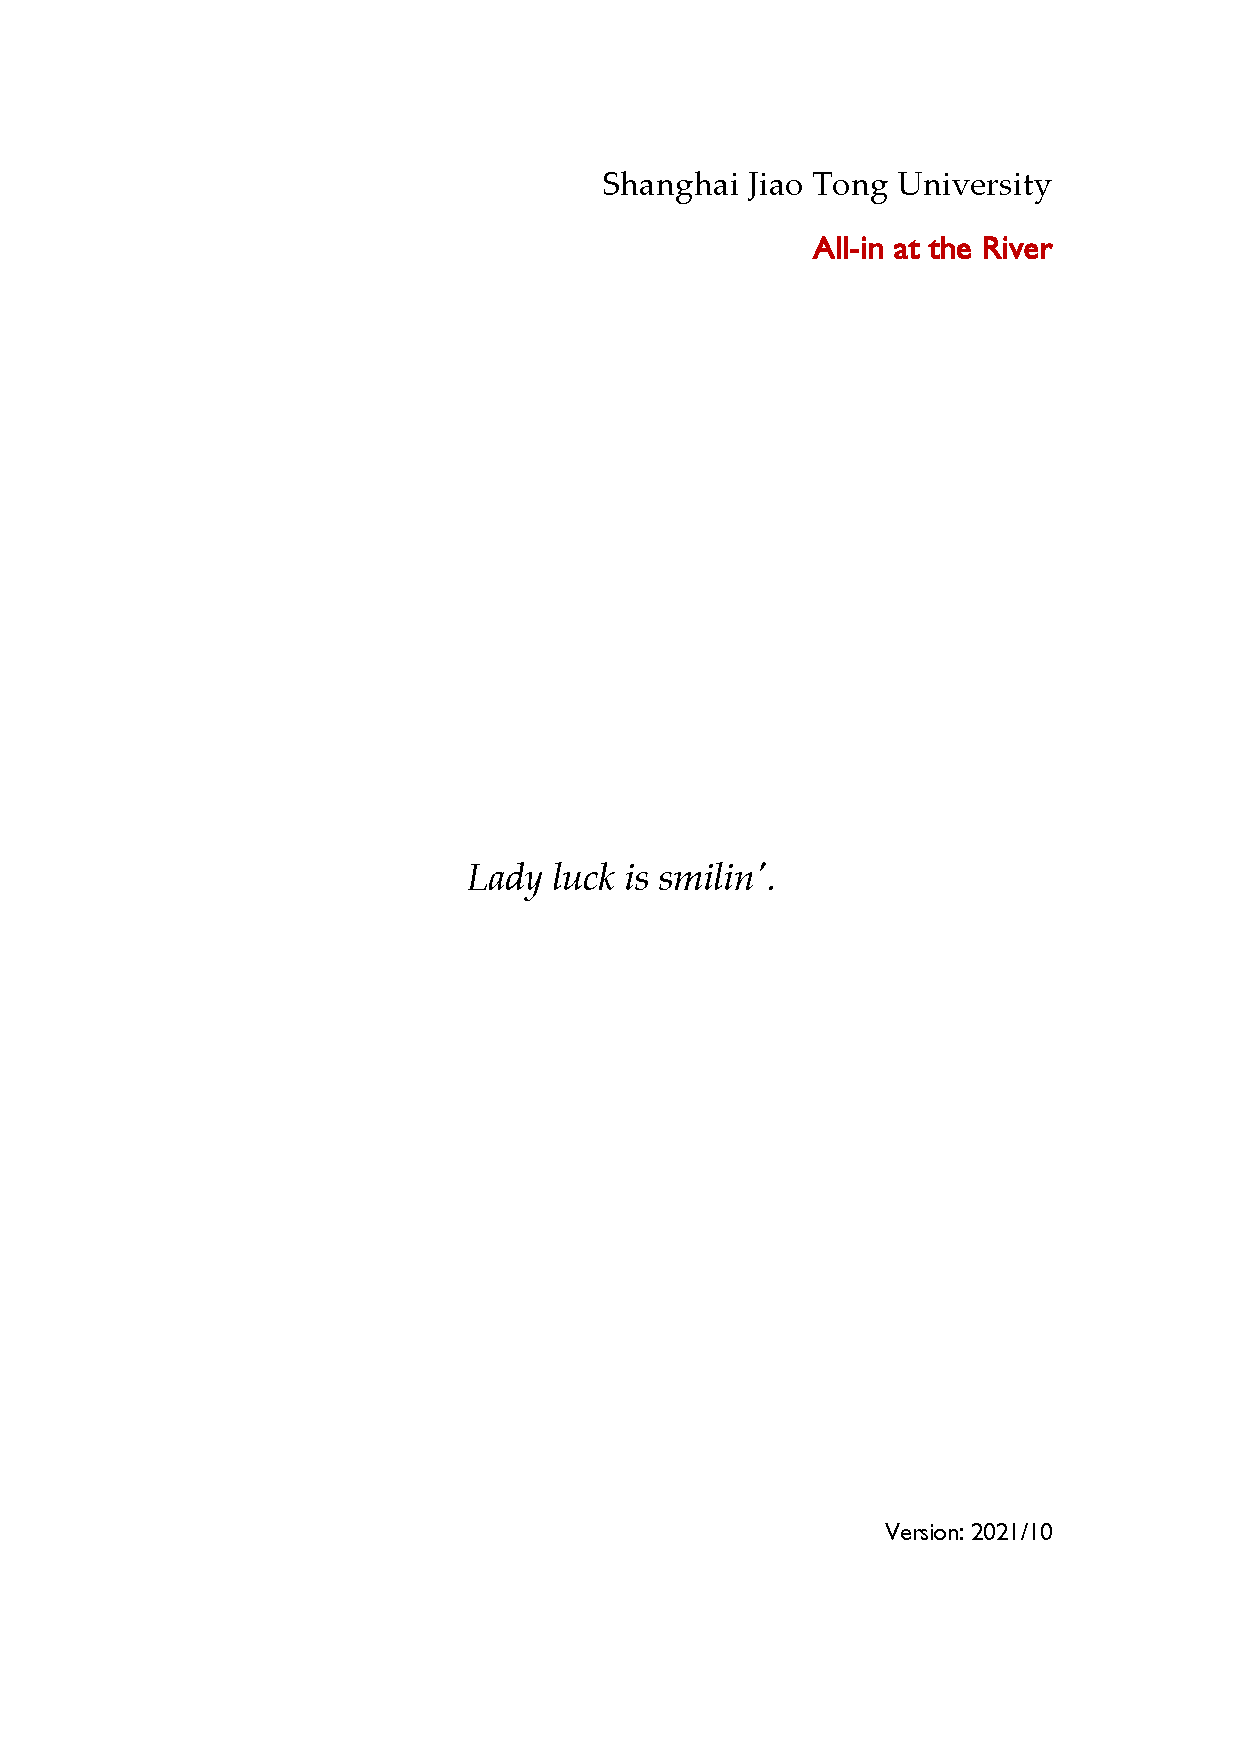
\includepdf{cover-back.pdf}
		\newpage
	\end{titlepage}
	\begin{multicols}{2}
		\setcounter{tocdepth}{2}
		\begingroup
		\let\cleardoublepage\relax
		\let\clearpage\relax
		\tableofcontents
		%\newpage
		\begin{spacing}{0.6}
			
			\section{Geometry}
				\subsection{凸包\checkmark}
				\inputminted{cpp}{src/Geometry/凸包.cpp}
				\subsection{闵可夫斯基和\checkmark}
				\inputminted{cpp}{src/Geometry/闵可夫斯基和.cpp}
				\subsection{最小覆盖圆}
				\inputminted{cpp}{src/Geometry/最小覆盖圆.cpp}
				\subsection{二维几何基础操作\checkmark}
				\inputminted{cpp}{src/Geometry/geo.cpp}
				\subsection{直线半平面交\checkmark}
				\inputminted{cpp}{src/Geometry/半平面交.cpp}
				\subsection{凸包快速询问\checkmark}
				\inputminted{cpp}{src/Geometry/logconvexhull.cpp}
%				\subsection{直线与凸包交点}
%				\inputminted{cpp}{src/Geometry/直线与凸包交点.cpp}
%				\subsection{点到凸包切线}
%				\inputminted{cpp}{src/Geometry/点到凸包切线.cpp}
%				\subsection{Delaunay 三角剖分}
%				\inputminted{cpp}{src/Geometry/DelaunayTriangulation.cpp}
				\subsection{三相之力\checkmark}
				\inputminted{cpp}{src/Geometry/三角形.cpp}
				\subsection{圆并}
				\inputminted{cpp}{src/Geometry/圆并.cpp}
				\subsection{多边形与圆交}
				\inputminted{cpp}{src/Geometry/多边形和圆的交.cpp}
				\subsection{阿波罗尼茨圆}
				\inputminted{cpp}{src/Geometry/阿波罗尼茨圆.tex}
				\subsection{圆幂 圆反演 根轴}
				\noindent
圆幂: 半径为 $R$ 的圆 $O$, 任意一点 $P$ 到 $O$ 的幂为 $h=OP^2-R^2$\\
圆幂定理: 过 $P$ 的直线交圆在 $A$ 和 $B$ 两点, 则 $PA\cdot PB=|h|$\\
根轴: 到两圆等幂点的轨迹是一条垂直于连心线的直线\\
反演: 已知一圆 $C$, 圆心为 $O$, 半径为 $r$, 如果 $P$与 $P'$在过圆心 $O$的直线上, 且 $OP\cdot OP'=r^2$, 则称 $P$与 $P'$关于 $O$互为反演. 一般 $C$取单位圆.\\
反演的性质: \\
不过反演中心的直线反形是过反演中心的圆, 反之亦然.\\
不过反演中心的圆, 它的反形是一个不过反演中心的圆.\\
两条直线在交点 $A$的夹角, 等于它们的反形在相应点 $A'$的夹角, 但方向相反.\\
两个相交圆周在交点 $A$的夹角等于它们的反形在相应点 $A'$的夹角, 但方向相反.\\
直线和圆周在交点 $A$的夹角等于它们的反演图形在相应点 $A'$的夹角, 但方向相反.\\
正交圆反形也正交. 相切圆反形也相切, 当切点为反演中心时, 反形为两条平行线. \\
				\subsection{球面基础}
				\noindent
球面距离: 连接球面两点的大圆劣弧 (所有曲线中最短)\\
球面角: 球面两个大圆弧所在半平面形成的二面角\\
球面凸多边形: 把一个球面多边形任意一边向两方无限延长成大圆, 其余边都在此大圆的同旁.\\
球面角盈$E$: 球面凸n边形的内角和与$(n-2)\pi$的差\\
离北极夹角$\theta$, 距离$h$的球冠: $S=2\pi Rh=2\pi R^2(1-\cos\theta)$, $V=\frac{\pi h^2}{3}(3R-h)$\\
球面凸n边形面积: $S=ER^2$\\
				\subsection{经纬度球面距离\checkmark}
				\inputminted{cpp}{src/Geometry/经纬度求球面最短距离.cpp}
%				\subsection{最近点对}
%				\inputminted{cpp}{src/Geometry/最近点对.cpp}
				\subsection{长方体表面两点最短距离}
				\inputminted{cpp}{src/Geometry/长方体表面两点最短距离.cpp}
				\subsection{圆上整点\checkmark}
				\inputminted{cpp}{src/Geometry/圆上整点.cpp}
				\subsection{相关公式}
				\begin{small}
\begin{spacing}{0.5}
\begin{multicols*}{2}
	\subsubsection{Heron's Formula}
	\begin{eqnarray*}
		&& S=\sqrt{p(p-a)(p-b)(p-c)} \\
		&& p=\frac{a+b+c}{2}
	\end{eqnarray*}
\subsubsection{四面体内接球球心}
假设$s_i$是第$i$个顶点相对面的面积,则有
\[\left\{
\begin{aligned}
x \ = \ \frac{s_1x_1+s_2x_2+s_3x_3+s_4x_4}{s_1+s_2+s_3+s_4}\\
y \ = \ \frac{s_1y_1+s_2y_2+s_3y_3+s_4y_4}{s_1+s_2+s_3+s_4}\\
z \ = \ \frac{s_1z_1+s_2z_2+s_3z_3+s_4z_4}{s_1+s_2+s_3+s_4}\\
\end{aligned}\right.\]
体积可以使用$1/6$混合积求, 内接球半径为
\[
r \ = \ \frac{3V}{s_1+s_2+s_3+s_4} \\
\]
\subsubsection{三角形内心}
	\[ \frac{a\vec {A} + b\vec{B} + c\vec{C}}{a + b + c} \]
\subsubsection{三角形外心}
	\[ \frac{\vec{A} + \vec{B} - \frac{\overrightarrow {BC} \cdot \overrightarrow{CA}}{\overrightarrow {AB} \times \overrightarrow{BC}}\overrightarrow {AB}^T}{2} \]
\subsubsection{三角形垂心}
	\[ \vec{H} = 3\vec{G} - 2\vec{O} \]
\subsubsection{三角形偏心}
	\[ \frac{-a\vec {A} + b\vec{B} + c\vec{C}}{-a + b + c} \]
	剩余两点的同理. 
\subsubsection{三角形内接外接圆半径}
	\[ r=\frac{2S}{a+b+c},\, R=\frac{abc}{4S} \]
\end{multicols*}
\subsubsection{Pick's Theorem}
\begin{eqnarray*}
S=I+\frac{B}{2}-1
\end{eqnarray*}
$S$ is the area of lattice polygon, $I$ is the number of lattice interior points, and $B$ is the number of lattice boundary points.
\subsubsection{Euler's Formula}
For convex polyhedron: $V-E+F=2$. \\
For planar graph: $|F|=|E|-|V|+n+1$, $n$ denotes the number of connected components.
\subsection{三角公式}
\noindent
\[
\sin(a \pm b) = \sin a \cos b \pm \cos a \sin b
\]
\[
\cos(a \pm b) = \cos a \cos b \mp \sin a \sin b
\]
\[
\tan(a \pm b) = \frac{\tan(a)\pm\tan(b)}{1 \mp \tan(a)\tan(b)}
\]
\[
\tan(a) \pm \tan(b) = \frac{\sin(a \pm b)}{\cos(a)\cos(b)}
\]
\[
\sin(a) + \sin(b) = 2\sin(\frac{a + b}{2})\cos(\frac{a - b}{2})
\]
\[
\sin(a) - \sin(b) = 2\cos(\frac{a + b}{2})\sin(\frac{a - b}{2})
\]
\[
\cos(a) + \cos(b) = 2\cos(\frac{a + b}{2})\cos(\frac{a - b}{2})
\]
\[
\cos(a) - \cos(b) = -2\sin(\frac{a + b}{2})\sin(\frac{a - b}{2})
\]
$
\sin(na) = n\cos^{n-1}a\sin a - \binom{n}{3}\cos^{n-3}a \sin^3a + \binom{n}{5}\cos^{n-5}a\sin^5a - \dots
$
\[
\cos(na) = \cos^{n}a - \binom{n}{2}\cos^{n-2}a \sin^2a + \binom{n}{4}\cos^{n-4}a\sin^4a - \dots
\]
\subsubsection{超球坐标系}
\begin{eqnarray*}
 	x_1 &=& r\cos(\phi_1) \\ 
	x_2 &=& r\sin(\phi_1)\cos(\phi_2) \\
%	x_3 &=& r\sin(\phi_1)\sin(\phi_2)\cos(\phi_3) \\
	\cdots\\
	x_{n-1} &=& r\sin(\phi_1)\cdots\sin(\phi_{n-2})\cos(\phi_{n-1}) \\
	x_n &=& r\sin(\phi_1)\cdots\sin(\phi_{n-2})\sin(\phi_{n-1}) \\
	\phi_{n-1} &\in& [0,2\pi]\\
	\forall {i=1..{n-1}}\phi_i &\in& [0,\pi]\\
\end{eqnarray*}
\subsubsection{三维旋转公式}
绕着$(0,0,0)-(ux,uy,uz)$旋转$\theta$, $(ux,uy,uz)$ 是单位向量
\[
R = \begin{smallmatrix} \cos \theta +u_x^2 \left(1-\cos \theta\right) \quad u_x u_y \left(1-\cos \theta\right) - u_z \sin \theta \quad u_x u_z \left(1-\cos \theta\right) + u_y \sin \theta \\ u_y u_x \left(1-\cos \theta\right) + u_z \sin \theta \quad \cos \theta + u_y^2\left(1-\cos \theta\right) \quad u_y u_z \left(1-\cos \theta\right) - u_x \sin \theta \\ u_z u_x \left(1-\cos \theta\right) - u_y \sin \theta \quad u_z u_y \left(1-\cos \theta\right) + u_x \sin \theta \quad \cos \theta + u_z^2\left(1-\cos \theta\right) 
\end{smallmatrix}.
\]
\[
\begin{bmatrix}
x' \\
y' \\
z' \\
\end{bmatrix} = R
\begin{bmatrix}
x \\
y \\
z \\
\end{bmatrix}
\]
\subsubsection{立体角公式}
\[ \phi \text{ : 二面角}\] 
\[ \Omega = \left(\phi_{ab} + \phi_{bc} + \phi_{ac}\right)\,\mathrm{rad} - \pi\,\mathrm{sr} \]\\
\[\tan \left( \frac{1}{2} \Omega/\mathrm{rad} \right) =
  \frac{\left|\vec a\ \vec b\ \vec c\right|}{abc + \left(\vec a \cdot \vec b\right)c + \left(\vec a \cdot \vec c\right)b + \left(\vec b \cdot \vec c\right)a}\]\\
\[\theta_s = \frac {\theta_a + \theta_b + \theta_c}{2}\]\\
\subsubsection{常用体积公式}
\begin{itemize}
\item Pyramid $V=\frac{1}{3}Sh$.
\item Sphere $V=\frac{4}{3}\pi R^3$.
\item Frustum $V=\frac{1}{3}h(S_1+\sqrt {S_1S_2}+S_2)$.
% \item Ellipsoid \\
% For ellipsoid with the standard equation in a Cartesian coordinate system $\frac{(x-x_0)^2}{a^2}+\frac{(y-y_0)^2}{b^2}+\frac{(z-z_0)^2}{c^2}=1$, $V=\frac{4}{3} \pi abc$.
\item Ellipsoid $V=\frac{4}{3} \pi abc$.
% \item Tetrahedron \\
% For tetrahedron $O-ABC$, let $a=AB,b=BC,c=CA,d=OC,e=OA,f=OB$, ${(12V)}^2=a^2d^2(b^2+c^2+e^2+f^2-a^2-d^2)+b^2e^2(c^2+a^2+f^2+d^2-b^2-e^2)+c^2f^2(a^2+b^2+d^2+e^2-c^2-f^2)-a^2b^2c^2-a^2e^2f^2-d^2b^2f^2-d^2e^2c^2$.
\end{itemize}
\subsubsection{高维球体积}
\begin{eqnarray*}
&& V_2=\pi R^2,\, S_2=2\pi R \\
&& V_3=\frac{4}{3}\pi R^3,\, S_3=4\pi R^2 \\
&& V_4=\frac{1}{2}\pi ^2 R^4,\, S_4=2\pi ^2 R^3 \\
%&& V_5=\frac{8}{15}\pi ^2 R^5,\, S_5=\frac{8}{3}\pi ^2 R^4 \\
%&& V_6=\frac{1}{6}\pi ^3 R^6,\, S_6=\pi ^3 R^5 \\
&& \mathrm{Generally}, V_n=\frac{2\pi}{n}V_{n-2},\, S_{n-1}=\frac{2\pi}{n-2}S_{n-3} \\
&& \mathrm{Where}, S_0=2,\, V_1=2,\, S_1=2\pi ,\, V_2=\pi
\end{eqnarray*}
\end{spacing}
\end{small}
				\newpage
				\subsection{三维几何基础操作\checkmark}
				\inputminted{cpp}{src/Geometry/三维几何.cpp}
				\subsection{三维凸包\checkmark}
				\inputminted{cpp}{src/Geometry/三维凸包.cpp}
				\subsection{最小覆盖球}
				\inputminted{cpp}{src/Geometry/最小覆盖球.cpp}
				\newpage
				
			%\begin{comment}
			
			%\section{Data Structure}
			%	\subsection{KD 树}
			%	\inputminted{cpp}{src/DataStructure/KD tree.cpp}
			%	\subsection{LCT 动态树}
			%	\inputminted{cpp}{src/DataStructure/LCT.cpp}
				%\subsection{可持久化平衡树}
				%\inputminted{cpp}{src/DataStructure/可持久化平衡树.cpp}
				% \subsection{有旋 Treap}
				% \inputminted{cpp}{src/DataStructure/有旋treap.cpp}
				
			\section{Tree \& Graph}
				\subsection{Hopcroft-Karp $O(\sqrt{|V|} |E|)$\checkmark}
				\inputminted{cpp}{src/TreeandGraph/Hopcroft.cpp}
				\subsection{Hungarian $O(|V| |E|)$\checkmark}
				\inputminted{cpp}{src/TreeandGraph/Hungarian.cpp}
				\subsection{Shuffle 一般图最大匹配 $O(|V| |E|)$\checkmark}
				\inputminted{cpp}{src/TreeandGraph/一般图最大匹配-shuffle.cpp}
				\subsection{极大团计数\checkmark}
				\inputminted{cpp}{src/TreeandGraph/CliqueCount.cpp}
				\subsection{有根树同构 Hash\checkmark}
				\inputminted{cpp}{src/TreeandGraph/TreeHash.cpp}
				\subsection{KM 最大权匹配 $O(|V|^3)$}
				\inputminted{cpp}{src/TreeandGraph/KM.cpp}
				%\subsection{Blossom 一般图带权最大匹配 $O(|V|^3)$}
				%\inputminted{cpp}{src/TreeandGraph/Blossom.cpp}
				\subsection{Tarjan 点双,边双}
				\inputminted{cpp}{src/TreeandGraph/Tarjan.cpp}
				\subsection{2-SAT\checkmark}
				\inputminted{cpp}{src/TreeandGraph/2-sat.cpp}
				\subsection{Dominator Tree 支配树\checkmark}
				\inputminted{cpp}{src/TreeandGraph/支配树.cpp}
				%\subsection{最大团}
				%\inputminted{cpp}{src/TreeandGraph/MaximumClique.cpp}
				\subsection{Minimum Mean Cycle}
				\inputminted{cpp}{src/TreeandGraph/MeanCycle.cpp}
				\subsection{弦图\checkmark}
				\begin{enumerate}
\item[1.] 团数 $\leq$ 色数 , 弦图团数 = 色数

\item[2.] 设 $next(v)$ 表示 $N(v)$ 中最前的点 . 
令 w* 表示所有满足 $A \in B$ 的 w 中最后的一个点 , 
判断 $v \cup N(v)$ 是否为极大团 , 
只需判断是否存在一个 w, 
满足 $Next(w)=v$ 且 $|N(v)| + 1 \leq |N(w)|$ 即可 . 

\item[3.] 最小染色 : 完美消除序列从后往前依次给每个点染色 , 
给每个点染上可以染的最小的颜色

\item[4.] 最大独立集 : 完美消除序列从前往后能选就选

\item[5.] 弦图最大独立集数 $=$ 最小团覆盖数 , 
最小团覆盖 : 
设最大独立集为 $\{p_1,p_2, \dots ,p_t\}$, 
则 $\{p_1\cup N(p_1), \dots , p_t \cup N(p_t)\}$ 
为最小团覆盖
\end{enumerate}

				\inputminted{cpp}{src/TreeandGraph/弦图.cpp}
				\subsection{欧拉回路\checkmark}
				\inputminted{cpp}{src/TreeandGraph/欧拉回路.cpp}
				\subsection{斯坦纳树}
				\inputminted{cpp}{src/TreeandGraph/斯坦纳树.cpp}
				\subsection{Dinic 最大流}
				\paragraph{复杂度证明思路}
假设 $\mathrm{dist}$ 为残量网络上的距离.
Dinic 一轮增广会找到一个极大的长度为 $\mathrm{dist} (s, t)$ 的增广路集合, 称为 blocking flow.
增广 blocking flow 后 $\mathrm{dist} (s, t)$ 将会增大.
因此, 最多只有 $O(V)$ 轮, 如果一轮增广是 $O(VE)$ 的,
那么总复杂度是 $O(V^2E)$.

注意, 没有当前弧优化的 Dinic 复杂度应是指数级别的.

\paragraph{单位流量网络}
在 0-1 流量图上 Dinic 有更好的性质. 
\begin{itemize}
	\setlength{\itemsep}{1pt}
	\setlength{\parskip}{0pt}
	\setlength{\parsep}{0pt}
	\item 复杂度为 $O(\min \{V ^ {2/3}, E ^ {1/2}\} E)$.
	\item $\mathrm{dist} (s, t) = d$, 残量网络上至多还存在 $E/d$ 的流.
	\item 如果是每个点只有一个入/出度, 复杂度 $O(V ^ {1 /2 } E)$. 一个著名的特殊情况是 Hopcroft-Karp.
\end{itemize}

				\inputminted{cpp}{src/TreeandGraph/Dinic.cpp}
				\subsection{Dijkstra 费用流\checkmark}
				\inputminted{cpp}{src/TreeandGraph/MCMF_dij.cpp}
				%\subsection{K短路}
				%\inputminted{cpp}{src/TreeandGraph/K短路.cpp}
				%\subsection{动态 MST}
				%\inputminted{cpp}{src/TreeandGraph/完全动态MST.cpp}
				%\subsection{三元环}
				%\inputminted{cpp}{src/TreeandGraph/三元环.cpp}
				%\subsection{平面图转对偶图}
				%\inputminted{cpp}{src/TreeandGraph/平面图转对偶图.cpp}
				%\subsection{最小乘积生成树}
				%\inputminted{cpp}{src/TreeandGraph/最小乘积生成树.cpp}
				%\subsection{树同构}
				%\inputminted{cpp}{src/TreeandGraph/树同构.cpp}
				%\subsection{树点分治 ??}
				%\inputminted{cpp}{src/TreeandGraph/点分治.cpp}
				%\subsection{虚树}
				%\inputminted{cpp}{src/TreeandGraph/虚树.cpp}
				%\subsection{动态最小生成树}
				%\inputminted{cpp}{src/TreeandGraph/DynamicMST.cpp}
				\subsection{Gomory-Hu 无向图最小割树 $O(n ^ 3 m)$}
				每次随便找两个点 $s, t$ 求在\textbf{原图}的最小割, 在最小割树上连 $(s, t, w_\mathrm{cut})$,
递归对由割集隔开的部分继续做. 在得到的树上, 两点最小割即为树上瓶颈路.
实现时, 由于是随意找点, 可以写为分治的形式.
				\subsection{Stoer-Wagner 无向图最小割 $O(nm + n ^ 2 \log n)$}
				\inputminted{cpp}{src/yzh/Stoer-Wagner.cpp}
				%\subsection{Cactus 仙人掌}
				%\inputminted{cpp}{src/TreeandGraph/cactus.cpp}
				\subsection{网络流总结}

\subsubsection{最小割集, 最小割必须边以及可行边}
\noindent

\textbf{最小割集} 从S出发, 在残余网络中BFS所有权值非0的边(包括反向边),得到点集$\{S\}$, 另一集为$\{V\} - \{S\}$. \\
\textbf{最小割集必须点} 残余网络中S直接连向的点必在S的割集中, 直接连向T的点必在T的割集中; 若这些点的并集为全集, 则最小割方案唯一.\\
\textbf{最小割可行边} 在残余网络中求强联通分量, 将强联通分量缩点后, 剩余的边即为最小割可行边, 同时这些边也必然满流.\\
\textbf{最小割必须边} 在残余网络中求强联通分量, 若S出发可到u, T出发可到v, 等价于$scc_S=scc_u$且$scc_T = scc_v$, 则该边为必须边.\\

\subsubsection{最大权闭合子图}
\noindent
适用问题: 每个点有点权, 限制条件形如: 选择A则必须选择B, 选择B则必须选择C, D. 建图方式: B向A连边, CD向B连边.\\
求解: S向正权点连边, 负权点向T连边, 其余边容量inf, 求最小割, 答案为S所在最小割集.

\subsubsection{二元关系}
\noindent
适用问题: 有$n$个元素, 每个元素可选A或者B, 各有代价; 有$m$个限制条件, 若元素$i$与$j$的种类不同则产生额外的代价, 求最小代价.\\
求解: S向i连边$A_i$, i向T连边$B_i$, 一组限制$(i,j)$代价为$z$, 则i与j之间连双向容量为$z$的边, 求最小割.

\subsubsection{二分图最小点覆盖和最大独立集}
\noindent
最小点覆盖: 求出一个最大匹配, 从左部开始每次寻找一个未匹配点, 从该点出发可以得到``未匹配-匹配-未匹配..."形式的交错树, 标记所有这些点. 则最小点覆盖方案为右部未标记点与左部标记点的并集. 显然最小点覆盖集合大小 = 最大匹配.\\
最大独立集 = 全集 - 最小点覆盖.

\subsubsection{整数线性规划转费用流}
\noindent
首先将约束关系转化为所有变量下界为$0$, 上界没有要求, 并满足一些等式,
每个变量在均在等式左边且出现恰好两次, 系数为$+1$和$-1$, 优化目标为$\max\sum v_ix_i$的形式.
将等式看做点, 等式i右边的值$b_i$若为正, 则$S$向$i$连边$(b_i, 0)$, 否则i向T连边$(-b_i, 0)$.
将变量看做边, 记变量$x_i$的上界为$m_i$(无上界则$m_i=inf$), 将$x_i$系数为$+1$的那个等式$u$向系数为$-1$的等式$v$连边$(m_i, v_i)$.
				\subsection{图论结论}
				\subsubsection{最小乘积问题原理}
\noindent
每个元素有两个权值{x_i}和{y_i}, 要求在某个限制下(例如生成树, 二分图匹配)使得{\Sigma x \Sigma y}最小.对于任意一种符合限制的选取方法, 记$X=\Sigma x_i$, $Y=\Sigma y_i$, 可看做平面内一点$(X,Y)$. 答案必在下凸壳上, 找出该下凸壳所有点, 即可枚举获得最优答案. 可以递归求出此下凸壳所有点, 分别找出距x, y轴最近的两点A, B, 分别对应于$\Sigma y_i$, $\Sigma x_i$最小. 找出距离线段最远的点C, 则C也在下凸壳上, C点满足$AB\times AC$最小, 也即$(X_B-X_A)Y_C + (Y_A-Y_B)X_C - (X_B-X_A)Y_A - (Y_B-Y_A)X_A$最小. 后两项均为常数, 因此将所以权值改成$(X_B-X_A)y_i+(Y_B-Y_A)x_i$,求同样问题(例如最小生成树, 最小权匹配)即可. 求出C点以后, 递归AC, BC.

				\subsubsection{最小环}
\noindent
无向图最小环: 每次floyd到k时, 判断1到k-1的每一个i,j: $ans = min\{ans, d(i,j)+map(i,k)+map(k,j)\}$, 然后再松弛k.\\
有向图最小环: 做完floyd后, $d(i,i)$即为经过i的最小环.
				\subsubsection{度序列的可图性}
\noindent
判断一个度序列是否可转化为简单图, 除了一种贪心构造的方法外, 下列方法更快速.
EG定理: 将度序列从大到小排序得到$\{d_i\}$, 此序列可转化为简单图当且仅当 $\Sigma d_i$为偶数, 且对于任意的$1\le k \le n-1$满足$\sum_{i=1}^{k} d_i \le k(k-1)+\sum_{i=k+1}^n \min(k, d_i)$.

				\subsection{切比雪夫距离与曼哈顿距离转化}
曼哈顿距离转切比雪夫距离:$(x,y)$->$(x+y,x-y)$, 适用于一些每次只能向四联通的格子走一格的问题.\\
切比雪夫距离转曼哈顿距离:$(x,y)$->$(\frac{x+y}{2}, \frac{x-y}{2})$, 适用于一些统计距离的问题.

				%\subsection{图论知识 - Nightfall}
				\begin{comment}
\subsubsection{完全动态MST}\
    一个$N$个点$M$条边的无向图, 每次可以修改任意一条边的权值, 在每个修改操作后输出当前最小生成树的边权和. $N,M,Q\leq50000$. 
    \par 我们假设, 有一个图$\{S\}$, 有$k$条边在之后会被修改. 在$k$个MST中, 有些边永远出现在这些MST 中, 而有些边永远不会出现在这些MST中. 我们可以尝试求出这些边, 从而缩小图的规模. 
    \paragraph{找出无用边}将需要修改的边标记为$\infty$, 然后跑MST, 这时不在MST上的且值不为$\infty$边必为无用边, 删除这些边, 减少边数 (注意还原) . 
    \paragraph{找出必须边}将需要修改的边标记为$-\infty$, 然后跑MST, 这时在MST上且不为$-\infty$的边为必须边, 将这些边连接的点合并, 缩小点集 (注意还原) . 
    \par 假设当前区间内需要修改的边数为$k$, 进行删去无用边和找出必须边操作后, 图中最多剩下$k+1$个点和$2k$条边. 如果每次都暴力求MST, 那么时间复杂度为$O(nlg^2n)$; 如果利用排好序的边求MST, 并使用路径压缩+按秩合并的并茶集, 那么时间复杂度为$O(nlgn\alpha (n))$. 
\end{comment}

\subsubsection{LCT常见应用}
                \paragraph{动态维护边双}\
                    可以通过LCT来解决一类动态边双连通分量问题. 即静态的询问可以用边双连通分量来解决, 而树有加边等操作的问题. 
                    \par 把一个边双连通分量缩到LCT的一个点中, 然后在LCT上求出答案. 缩点的方法为加边时判断两点的连通性, 如果已经联通则把两点在目前LCT路径上的点都缩成一个点. 
                \paragraph{动态维护基环森林}\
                    通过LCT可以动态维护基环森林, 即每个点有且仅有一个出度的图. 有修改操作, 即改变某个点的出边. 对于每颗基环森林记录一个点为根, 并把环上额外的一条边单独记出, 剩下的边用LCT维护. 一般使用有向LCT 维护. 
                    \par 修改时分以下几种情况讨论: 1, 修改的点是根, 如果改的父亲在同一个联通块中, 直接改额外边, 否则删去额外边, 在LCT上加边. 2, 修改的点不是根, 那么把这个点和其父亲的联系切除. 如果该点和根在一个环上, 那么把多的那条边加到LCT上. 最后如果改的那个父亲和修改的点在一个联通块中, 记录额外边, 否则LCT上加边. 具体见例题. 
\subsubsection{LCT解决子树询问}\
                通过记录轻边信息可以快速地维护出整颗LCT的一些值. 如子树和, 子树最大值等. 在Access时要进行虚实边切换, 这时减去实边的贡献, 并加上新加虚边的贡献即可. 有时需要套用数据结构, 如Set来维护最值等问题. 
                \par 模板: 1, $x\to y$链$+z$; 2, $x\to y$链变为$z$; 3, 在以$x$为根的树对$y$子树的点权求和; 4, $x\to y$ 链取$max$; 5, $x\to y$链求和; 6, 连接$x~y$; 7, 断开$x~y$. 保证操作合法. 
                \par $V$单点值; $sz$平衡树的$SZ$; $mv$链上最大; $S$链上和; $sm$ 区间相同标记; $lz$区间加标记; $B$ 虚边之和; $ST$子树信息和; $SM$子树+链上信息和. 更新时, $S[x]=S[c[x][0]]+S[c[x][1]]+V[x]$,   $ST[x]=B[x]+ST[c[x][0]]+ST[c[x][1]]$, $SM[x]=S[x]+ST[x]$. 

\subsubsection{差分约束}若要使得所有量两两的值最接近, 则将如果将源点到各点的距离初始化为$0$.  若要使得某一变量与其余变量的差最大, 则将源点到各点的距离初始化为$∞$, 其中之一为$0$.  若求最小方案则跑最长路, 否则跑最短路. 

\subsubsection{斯坦纳树}\
		在一个无向带权图$G=(V,E)$中, 将指定的$k$个点连通的一颗树称为\textbf{斯坦纳树}, 边权总和最小的斯坦纳树称为最小斯坦纳树. 
		\par 我们可以用DP+SPFA的方法求解斯坦纳树. 用$F_{i,state}$表示以$i$为根, 指定集合中的点的联通状态为$state$的生成树的最小总权值, 有两种转移方程. 
		\par 第一种, 通过两个子集合并进行转移, 即$F_{i,state}=min(F_{i,subset1} + F_{i,subset2})$, 这一部分使用DP完成. 
		\par 第二种, 在当前的联通状态下, 对该联通状态进行松弛操作, 即${F_{i,state}=min(F_{i,state},F_{j,state}+w(i,j))}$, 这一部分使用SPFA完成. 
        \par 时间复杂度$O(V*3^k+cE*2^k)$, $c$为SPFA复杂度中的常数. 

\subsubsection{李超线段树}\
        李超线段树可以动态在添加若干条线段或直线$(a_i,b_i)\to (a_j,b_j)$, 每次求$[l,r]$上最上面的那条线段的值. 思想是让线段树中一个节点只对应一条直线, 如果在这个区间加入一条直线, 那么分类讨论. 如果新加的这条直线在左右两端都比原来的更优, 则替换原来的直线, 将原来的直线扔掉. 如果左右两端都比原来的劣, 将这条直线扔掉. 如果一段比原来的优, 一段比原来的劣, 那么判断一下两条线的交点, 判断哪条直线可以完全覆盖一段一半的区间, 把它保留, 另一条直线下传到另一半区间. 时间复杂度$O(nlgn)$. 
\subsubsection{吉如一线段树}\
        吉如一线段树能解决一类区间和某个数取最大或最小, 区间求和的问题. 以区间取最小值为例, 在线段树的每一个节点额外维护区间中的最大值$ma$, 严格次大值$se$以及最大值个数$t$. 现在假设我们要让区间$[L,R]$对$x$取min, 先在线段树中定位若干个节点, 对于每个节点分三种情况讨论: 1, 当$ma\leq x$时, 显然这一次修改不会对这个节点产生影响, 直接退出; 2, 当$se<x<ma$时, 显然这一次修改只会影响到所有最大值, 所以把$num$加上$t*(x-ma)$, 把$ma$更新为$x$, 打上标记退出; 3, 当$se\geq x$时, 无法直接更新着一个节点的信息, 对当前节点的左儿子和右儿子递归处理. 单次操作均摊复杂度$O(lg^2n)$. 

\subsubsection{二分图最大匹配}
        \paragraph{最大独立集 最小覆盖点集 最小路径覆盖} 最大独立集指求一个二分图中最大的一个点集, 使得该点集内的点互不相连. \textbf{最大独立集=总顶点数-最大匹配数}. 最小覆盖点集指用最少的点, 使所有的边至少和一个点有关联. \textbf{最小覆盖点集=最大匹配数}. 最小路径覆盖指一个DAG图$G$中用最少的路径使得所有点都被经过. \textbf{最小路径覆盖=总点数-最大匹配数} (拆点构图). 最大独立集$S$与最小覆盖集$T$互补. 构造方法: 1.做最大匹配, 没有匹配的空闲点$u\in S$ 2.如果$u\in S$那么$u$的邻点必然属于$T$ 3.如果一对匹配的点中有一个属于$T$那么另外一个属于$S$ 4.还不能确定的, 把左子图的放入$S$, 右子图放入$T$.
        \paragraph{二分图最大匹配关键点} 关键点指的是一定在最大匹配中的点. 由于二分图左右两侧是对称的, 我们只考虑找左侧的关键点. 先求任意一个最大匹配, 然后给二分图定向: 匹配边从右到左, 非匹配边从左到右, 从左侧每个不在最大匹配中的点出发DFS, 给到达的那些点打上标记, 最终左侧每个没有标记的匹配点即将爱为关键点. 时间复杂度$O(n+m)$. 
        \paragraph{Hall定理}二分图$G=(X,Y,E)$有完备匹配的充要条件是: 对于$X$的任意一个子集$S$都满足$|S|leq |A(S)|$, $A(S)$是$Y$的子集, 是$S$的邻集. 邻集的定义是与$S$有边的点集. 

\subsubsection{稳定婚姻问题}\
         有$n$位男士和$n$位女士, 每个人都对每个异性有一个不同的喜欢程度, 现在使得每人恰好有一个异性配偶. 如果男士$u$和女士$v$不是配偶但喜欢对方的程度都大于喜欢各自当前的配偶, 则称他们为一个不稳定对. 稳定婚姻问题是为了找出一个不含不稳定对的方案. 
         \par 稳定婚姻问题的经典算法为求婚-拒绝算法, 即男士按自己喜欢程度从高到底依次向每位女士求婚, 直到有一个接受他. 女士遇到比当前配偶更差的男士时拒绝他, 遇到更喜欢的男士时就接受他, 并抛弃以前的配偶. 被抛弃的男士继续按照列表向剩下的女士依次求婚, 直到所有人都有配偶. 如果算法一定能得到一个匹配, 而且这个匹配一定是稳定的. 时间复杂度$O(n^2)$. 
\subsubsection{最大流和最小割}
	%\paragraph{最小割集求法} 从源点$S$出发, 在残量网络上走, 所有走到的点属于$S$集, 其余点属于$T$集. 
	\paragraph{常见建模方法} 拆点; 黑白染色; 流量正无穷表示冲突; 缩点; 数据结构优化建图; 最小割:每个变元拉一条$S$到$T$的链, 割在哪里表示取值, 相互连边表示依赖关系; 先把收益拿下, 在考虑冲突与代价的影响. 
	%\subparagraph{拆点} 如果一个点有经过次数限制, 可以将它拆成两个点: 一个入点和一个出点. 入点向出点连经过流量为次数限制的边, 然后出点向入点连边即可. 
	%\subparagraph{黑白染色} 一些图有隐含关系, 具有冲突的节点一定能黑白染色出来, 这样可以把黑点放在左部, 白点放在右部来解决问题. 
	%\subparagraph{用流量为正无穷的边表示冲突} 最小割建图中常用, 若左部一点和右部一点只能取一个或者至少取一个, 在它们之间连一条流量为正无穷的边. 
	%\subparagraph{缩点}几个节点的来源或者去向相同, 可以缩为同一个点. 如果从$u$到$v$有一条容量为$\infty$ 的边, 并且点$v$除了点$u$以外没有别的流量来源, 可以把这两个结点合并为一个. 
	%\subparagraph{数据结构优化建图}当一个点同时连一段点的时候, 可以用线段树, ST表等将一段点处理到一起连, 优化建图. 
	%\subparagraph{二者取其一式最小割}每个点都有两种方案可以选择, 每种方案都有一个花费, 并且只能选则其中一种. 另外如果某两个点选择了不同的方案, 还要在这两个点之间增加额外的费用. 新建$S$和$T$表示两种方案, 连边$(S,i,a_i)$或$(i,T,b_i)$表示支持哪一方, 每一对关系连边$(i,j,v_{i,j})$和$(j,i,v_{i,j})$, 求一次最小割即为结果. 
	%\subparagraph{最大权闭合子图/蕴含式最大获利问题}在一个有向图中, 每个点有一个可正可负的点权$a_i$, 对于任意一条有向边$(i,j)$, 如果选了$i$就必须选$j$, 选择一些点使权值最大. 对于点$i$, 如果$a_i$为正, 则连边$(S,i,a_i)$, 否则连边$(i,T,-a_i)$. 对于原图的边$(i,j)$, 连边$(i,j,\infty)$. 则最大权=正权和-最大流. 
	\paragraph{判断一条边是否可能/一定在最小割中}令$G'$为残量网络$G$在强联通分量缩点之后的图. 那么一定在最小割中的边$(u,v)$: $(u,v)$满流, 且在$G'$中$u=S,v=T$; 可能在最小割方案中的边$(u,v)$: $(u,v)$满流, 或$(u,v)$满流, 且在$G'$中$u\neq v$. 
	\paragraph{混合图欧拉回路}把无向边随便定向, 计算每个点的入度和出度, 如果有某个点出入度之差$deg_i=in_i-out_i$为奇数, 肯定不存在欧拉回路. 对于$deg_i>0$的点, 连接边$(i,T,deg_i/2)$;对于$deg_i<0$的点, 连接边$(S,i,-deg_i/2)$. 最后检查是否满流即可. 
	\subsubsection{一些网络流建图}
	\paragraph{无源汇有上下界可行流}\
	\par 每条边$(u,v)$ 有一个上界容量$C_{u,v}$和下界容量$B_{u,v}$, 我们让下界变为$0$,上界变为$C_{u,v}-B_{u,v}$, 但这样做流量不守恒. 建立超级源点$SS$和超级汇点$TT$, 用$du_i$来记录每个节点的流量情况, $du_i=\sum B_{j,i}-\sum B_{i,j}$, 添加一些附加弧. 当$du_i>0$时, 连边$(SS,i,du_i)$;当$du_i<0$时, 连边$(i,TT,-du_i)$. 最后对$(SS,TT)$求一次最大流即可, 当所有附加边全部满流时(即$maxflow==所有du_i>0之和$)时有可行解. 
	\paragraph{有源汇有上下界最大可行流}\
	\par 建立超级源点$SS$和超级汇点$TT$, 首先判断是否存在可行流, 用无源汇有上下界可行流的方法判断. 增设一条从$T$到$S$没有下界容量为无穷的边, 那么原图就变成了一个无源汇有上下界可行流问题. 同样地建图后, 对$(SS,TT)$进行一次最大流, 判断是否有可行解. 
	\par 如果有可行解, 删除超级源点$SS$和超级汇点$TT$, 并删去$T$ 到$S$的这条边, 再对$(S,T)$进行一次最大流, 此时得到的$maxflow$即为有源汇有上下界最大可行流. 
	\paragraph{有源汇有上下界最小可行流}\
	\par 建立超级源点$SS$和超级汇点$TT$, 和无源汇有上下界可行流一样新增一些边, 然后从SS到TT跑最大流. 接着加上边$(T,S,\infty)$, 再从$SS$到$TT$跑一遍最大流. 
	\par 如果所有新增边都是满的, 则存在可行流, 此时$T$到$S$这条边的流量即为最小可行流. 
	\paragraph{有上下界费用流}\
	\par 如果求无源汇有上下界最小费用可行流或有源汇有上下界最小费用最大可行流, 用1.6.3.1/1.6.3.2 的构图方法, 给边加上费用即可. 
	\par 求有源汇有上下界最小费用最小可行流, 要先用1.6.3.3的方法建图, 先求出一个保证必要边满流情况下的最小费用. 如果费用全部非负, 那么这时的费用就是答案. 如果费用有负数, 那么流多了可能更好, 继续做从$S$到$T$的流量任意的最小费用流, 加上原来的费用就是答案. 
	\paragraph{费用流消负环}
	\par 新建超级源SS汇TT, 对于所有流量非空的负权边e, 先流满(ans+=e.f*e.c, e.rev.f+=e.f, e.f=0), 再连边SS$\to$e.to, e.from$\to$TT, 流量均为e.f(>0), 费用均为0. 再连边T$\to$S流量$\infty$费用0. 此时没有负环了. 做一遍SS到TT的最小费用最大流, 将费用累加ans, 拆掉T$\to$S的那条边 (此边的流量为残量网络中S$\to$T的流量). 此时负环已消, 再继续跑最小费用最大流.
	\paragraph{二物流}
	\par 水源S1, 水汇T1, 油源S2, 油汇T2, 每根管道流量共用. 求流量和最大.\\
	建超级源SS1汇TT1, 连边SS1$\to$S1,SS1$\to$S2,T1$\to$TT1,T2$\to$TT1, 设最大流为x1.\\
	建超级源SS2汇TT2, 连边SS2$\to$S1,SS2$\to$T2,T1$\to$TT2,S2$\to$TT2, 设最大流为x2.\\
	则最大流中水流量$\frac{x1+x2}{2}$, 油流量$\frac{x1-x2}{2}$.

\subsubsection{割点于割边}
        \paragraph{割点 割边} 一个点$u$是割点, 当且仅当: 1. $u$为非树根且有树边$(u,v)$满足$dfn_u\leq low_v$; 2. u为树根且有多于一个的子树. 一条无向边$(u,v)$是桥, 当且仅当$(u,v)$是树边, 且满足$dfn_u<low_v$. 

\subsubsection{2-SAT}
    如果选$A$就必须选$B$就从$A$向$B$连一条边, 如果两个只能选一个的条件在同一个强连通分量中就不合法. 输出可行方案可以比较$X$和$X’$的$bl$的大小, 大的选$X’$. 建图优化一般考虑前后缀的合并. 

\subsubsection{弦图}
				\paragraph{定义}我们称连接环中不相邻的两个点的边为弦. 一个无向图称为弦图, 当图中任意长度都大于$3$ 的环都至少有一个弦. 弦图的每一个诱导子图一定是弦图. 
				\paragraph{单纯点}设$N(v)$表示与点$v$相邻的点集. 一个点称为单纯点当${v}+N(v)$的诱导子图为一个团. 引理: 任何一个弦图都至少有一个单纯点, 不是完全图的弦图至少有两个不相邻的单纯点. 
				\paragraph{完美消除序列}一个序列${v_1,v_2,...,v_n}$满足$v_i$在${v_i,v_{i+1},...,v_n}$的诱导子图中为一个单纯点. 一个无向图是弦图当且仅当它有一个完美消除序列. 
				\paragraph{最大势算法}最大势算法能判断一个图是否是弦图. 从$n$到$1$的顺序依次给点标号(标号为$i$ 的点出现在完美消除序列的第$i$个). 设$label_i$表示第$i$个点与多少个已标号的点相邻, 每次选择$label_i$最大的未标号的点进行标号. 
				\par 然后判断这个序列是否为完美序列. 如果依次判断${v_{i+1},...,.v_n}$ 中所有与$v_i$相邻的点是否构成一个团, 时间复杂度为$O(nm)$. 考虑优化, 设${v_{i+1},...,v_n}$中所有与$v_i$ 相邻的点依次为$v_{j1}$,...,$v_{jk}$.  只需判断$v_{j1}$是否与$v_{j2}$,...,$v_{jk}$相邻即可. 时间复杂度$O(n+m)$. 
				\paragraph{弦图的染色}按照完美消除序列中的点倒着给图中的点贪心染尽可能最小的颜色, 这样一定能用最少的颜色数给图中所有点染色. 弦图的团数=染色数. 
                \paragraph{最大独立集}完美消除序列从前往后能选就选. 最大独立集=最小团覆盖. 

\subsubsection{三元环}\
                有一种简单的写法, 对于每条无向边$(u,v)$, 如果$deg_u<deg_v$, 那么连有向边$(u,v)$, 否则连有向边$(v,u)$(注意度数相等以点标号为第二关键字判断). 然后枚举每个点$x$, 假设$x$ 是三元环中度数最小的点, 然后暴力往后面枚两条边找到点$y$, 判断是否有边$(x,y)$即可. 可以证明, 这样的时间复杂度也是为$O(m\sqrt{m})$的. 

\subsubsection{图同构}
                令$F_t(i)=(F_{t-1}(i)*A+\sum_{i\to j} F_{t-1}(j)*B+\sum_{j\to i} F_{t-1}(j)*C+D*(i-a))mod P$, 枚举点$a$, 迭代$K$次后求得的就是$a$点所对应的$hash$值, 其中$K,A,B,C,D,P$为$hash$参数, 可自选. 

\subsubsection{竞赛图存在 Landau’s Theorem}
    $n$个点竞赛图点按出度按升序排序, 前$i$个点的出度之和不小于$\frac{i(i-1)}{2}$, 度数总和等于$\frac{n(n-1)}{2}$. 否则可以用优先队列构造出方案.

\subsubsection{Ramsey Theorem}
    $6$个人中至少存在$3$人相互认识或者相互不认识. $R(3,3)=6, R(4,4)=18$

\subsubsection{树的计数 Prufer序列}
    树和其prufer编码一一对应, 一颗$n$个点的树, 其prufer编码长度为${n-2}$, 且度数为$d_i$ 的点在prufer 编码中出现${d_i -1}$次. 
    \par 由树得到序列: 总共需要$n-2$步, 第$i$步在当前的树中寻找具有最小标号的叶子节点, 将与其相连的点的标号设为Prufer序列的第$i$个元素$p_i$, 并将此叶子节点从树中删除, 直到最后得到一个长度为$n-2$的Prufer 序列和一个只有两个节点的树. 
    \par 由序列得到树: 先将所有点的度赋初值为$1$, 然后加上它的编号在Prufer序列中出现的次数, 得到每个点的度; 执行$n-2$步, 第$i$步选取具有最小标号的度为$1$的点$u$与$v=p_i$ 相连, 得到树中的一条边, 并将$u$和$v$ 的度减一. 最后再把剩下的两个度为$1$的点连边, 加入到树中. 
    \par 相关结论: $n$个点完全图, 每个点度数依次为$d_1$,$d_2$,...,$d_n$, 这样生成树的棵树为: ${\frac{(n-2)!}{(d_1-1)!(d_2-1)!...(d_n-1)!}}$.\\
    左边有$n_1$个点, 右边有$n_2$个点的完全二分图的生成树棵树为$n_1^{n_2-1}+n_2^{n_1-1}$. \\
    $m$个连通块, 每个连通块有$c_i$个点, 把他们全部连通的生成树方案数: $(\sum c_i)^{m-2}\prod c_i$
\subsubsection{有根树的计数}\noindent
    首先, 令$S_{n,j}=\sum_{1\leq j\leq n/j}$; 于是$n+1$个结点的有根树的总数为$ a_{n+1}=\frac{\sum_{j=1}^nja_jS_{n-j}}{n}$. 注: $a_1=1,a_2=1,a_3=2,a_4=4,a_5=9,a_6=20,a_9=286,a_11=1842$. 
\subsubsection{无根树的计数}\noindent
    当$n$是奇数时, 有$a_n-\sum_{i}^{n/2}a_ia_{n-i}$种不同的无根树. \\
    当$n$时偶数时, 有$a_n-\sum_{i}^{n/2}a_ia_{n-i}+\frac{1}{2}a_{n/2}(a_{n/2}+1)$种不同的无根树. 
\subsubsection{生成树计数 Kirchhoff's Matrix-Tree Thoerem}
    Kirchhoff Matrix $T=Deg-A$, $Deg$是度数对角阵, $A$是邻接矩阵. 无向图度数矩阵是每个点度数; 有向图度数矩阵是每个点入度.\\
    邻接矩阵$A[u][v]$表示$u$−>$v$边个数, 重边按照边数计算, 自环不计入度数.\\
    无向图生成树计数: $c=|K$的任意1个$n−1$阶主子式$|$\\
    有向图外向树计数: $c=|$去掉根所在的那阶得到的主子式$|$
\subsubsection{有向图欧拉回路计数 BEST Thoerem}
        \[ \mathrm{ec}(G) = t_w(G)\prod_{v \in{V}}(\mathrm{deg}(v) - 1)! \]
        其中$deg$为入度(欧拉图中等于出度), $t_w(G)$为以$w$为根的外向树的个数. 相关计算参考生成树计数.\\
        欧拉连通图中任意两点外向树个数相同: $\mathrm{t_v}(G) = \mathrm{t_w}(G)$.
%\subsubsection{Tutte Matrix}
%    Tutte matrix $A$ of a graph $G=(V,E)$ : 
%    \[A_{ij}=\left\{
%        \begin{aligned}
%            & x_{ij} & \text{if}(i,j)\in E \text{and}i<j
%            & -x_{ij} & \text{if}(i,j)\in E \text{and}i>j
%            & 0 & \text{otherwise}
%        \end{aligned}
%        \right.\]
%    where $x_{ij}$ are indeterminates. The determinant of this skew-symmetric matrix is then a polynomial (in the variables $x_{ij}$, $i<j$ ): this coincides with the square of the pfaffian of the matrix $A$ and is non-zero (as a polynomial) if and only if a perfect matching exists.
%\begin{comment}
    \subsubsection{Edmonds Matrix}
        Edmonds matrix $A$ of a balanced ($|U|=|V|$) bipartite graph $G=(U,V,E)$ : 
        \[A_{ij}=\left\{
            \begin{aligned}
                & x_{ij} & (u_i,v_j)\in E\\
                & 0 & (u_i,v_j)\notin E
            \end{aligned}
            \right.\]
        where the $x_{ij}$ are indeterminates. $G$有完美匹配当且仅当关于$x_{ij}$的多项式$det(A_{ij})$不恒为$0$.
        完美匹配的个数等于多项式中单项式的个数.
%\end{comment}
\subsubsection{Count Acyclic Orientations}
    \noindent
    The chromatic polynomial is a function $P_G(q)$ that counts the number of $q$-colorings of $G$.\\
    Triangle $K_3$ : $t(t-1)(t-2)$\\
    Complete graph $K_n$ : $t(t-1)(t-2)\cdots (t-(n-1))$\\
    Tree with $n$ vertices : $t(t-1)^{n-1}$\\
    Cycle $C_n$ : $(t-1)^{n}+(-1)^{n}(t-1)$\\
    The number of acyclic orientations of an $n$-vertex graph $G$ is $(−1)^nP_G(−1)$, where $P_G(q)$ is the chromatic polynomial of the graph
    $G$.

			
			\section{String}
				\subsection{最小表示法}
				\inputminted{cpp}{src/String/最小表示法.cpp}
				\subsection{Manacher}
				\inputminted{cpp}{src/String/Manacher.cpp}
				\subsection{Multiple Hash}
				\inputminted{cpp}{src/String/hash.cpp}	
				\subsection{KMP exKMP}
				\inputminted{cpp}{src/String/KMP.cpp}
				\subsection{AC 自动机}
				\inputminted{cpp}{src/String/AC 自动机.cpp}
				\subsection{Lydon Word Decomposition}
				\inputminted{cpp}{src/String/Lyndon Word.cpp}
				\subsection{后缀数组\checkmark}
				\inputminted{cpp}{src/String/SA.cpp}
				\subsection{后缀自动机}
				\inputminted{cpp}{src/String/SAM.cpp}
				\subsection{Suffix Balanced Tree 后缀平衡树}
				\inputminted{cpp}{src/String/后缀平衡树.cpp}
				%\subsection{Total LCS 子串对目标求 LCS}
				%\inputminted{cpp}{src/String/Total LCS.cpp}
				%\subsection{Palindrome Automation 回文自动机}
				%\inputminted{cpp}{src/String/PAM.cpp}
				\subsection{String Conclusions}
				\subsubsection{双回文串}
\noindent
如果$s=x_1x_2=y_1y_2=z_1z_2, |x_1|<|y_1|<|z_1|, x_2, y_1, y_2, z_1$是回文串, 则$x_1$和$z_2$也是回文串. 

\subsubsection{Border 和周期}
\noindent
如果$r$是$S$的一个border, 则$|S|-r$是$S$的一个周期.\\
如果$p$和$q$都是$S$的周期, 且满足$p+q\le |S|+gcd(p,q)$, 则$gcd(p,q)$也是一个周期.

\subsubsection{字符串匹配与Border}
\noindent
若字符串$S$, $T$满足$2|S|\ge |T|$, 则$S$在$T$中所有匹配位置成一个等差数列.\\
进一步地, 若$S$的匹配次数大于2, 则等差数列的周期恰好等于$S$的最小周期.

\subsubsection{Border 的结构}
\noindent
字符串$S$的所有不小于$|S|/2$的border长度组成一个等差数列.\\
字符串$S$的所有 border 按长度排序后可分成$O(\log{|S|})$段, 每段是一个等差数列. 

\subsubsection{回文串Border}
\noindent
回文串长度为$t$的后缀是一个回文后缀, 等价于$t$是该串的border. 因此回文后缀的长度也可以划分成$O(\log{|S|})$段.

\subsubsection{子串最小后缀}
\noindent
设$s[p..n]$是$s[i..n]$, $(l \leq i \leq r)$中最小者, 则minsuf(l, r)等于$s[p..r]$的最短非空 border. minsuf(l, r) = min\{$s[p..r]$, minsuf(r − $2^k$ + 1, r)\}, $(2^k < r − l + 1 \leq 2^{k+1})$. 

\subsubsection{子串最大后缀}
\noindent
从左往右扫, 用set维护后缀的字典序递减的单调队列, 并在对应时刻添加"小于事件"点以便在之后修改队列; 查询直接在set里lower\_bound. 
			
			\section{Math 数学}
				\subsection{exgcd}
				\inputminted{cpp}{src/Math/exgcd.cpp}
				\subsection{CRT 中国剩余定理}
				\inputminted{cpp}{src/Math/CRT_lbn.cpp}
				\subsection{扩展卢卡斯}
				\inputminted{cpp}{src/Math/扩展卢卡斯.cpp}
				\subsection{阶乘取模}
				\inputminted{cpp}{src/Math/Factorial Mod.cpp}
				\subsection{类欧几里得 直线下格点统计\checkmark}
				\inputminted{cpp}{src/Math/直线下格点统计.cpp}
				\subsection{平方剩余}
				\inputminted{cpp}{src/Math/平方剩余.cpp}
				\subsection{BSGS 离散对数}
				\inputminted{cpp}{src/Math/BSGS.cpp}
				\subsection{线性同余不等式}
				\inputminted{cpp}{src/Math/线性同余不等式.cpp}
				\subsection{Miller Rabin, Pollard Rho}
				\inputminted{cpp}{src/Math/Miller Rabin And Pollard Rho.cpp}
				% \subsection{杜教筛}
				% \inputminted{cpp}{src/Math/杜教筛.cpp}
				% \subsection{min25 筛}
				% \inputminted{cpp}{src/Math/TEES.cpp}
				\subsection{原根}
				% \inputminted{cpp}{src/Math/原根.cpp
				% \subsection{阶}

\paragraph{定义} 使得 $a^x \bmod m=1$ 的最小的x, 记作 $\delta_m(a)$.
若 $a\equiv g^s \mod m$, 其中 $g$ 为 $m$ 的一个原根.
则虽然 $s$ 随 $g$ 的不同取值有所不同, 但是必然满足 $\delta_m(a)=\gcd(s,\varphi(m))$.
\paragraph{性质} $\delta_m(a^k)=\frac{\delta_m(a)}{\gcd(\delta_m(a),k)}$
\paragraph{$k$ 次剩余} 给定方程 $x^k\equiv a \mod m$, 求所有解.
若 $k$ 与 $\varphi(m)$ 互质, 
则可以直接求出 $k$ 对 $\varphi(m)$ 的逆元.
否则, 将 $k$ 拆成两部分, $k=uv$,
其中 $u\bot \varphi(m)$, $v|\varphi(m)$,
先求 $x^v\equiv a \mod m$,
则 $ans=x^{u^{-1}}$.
下面讨论 $k|\varphi(m)$ 的问题.
任取一原根 $g$, 对两侧取离散对数,
设 $x=g^s$, $a=g^t$, 其中 $t$ 可以用BSGS求出,
则问题转化为求出所有的 $s$ 满足 $ks\equiv t \mod \varphi(m)$,
exgcd 即可求解, 显然有解的条件是 $k|\delta_m(a)$.

				\subsection{FFT NTT FWT 多项式操作}
				\inputminted{cpp}{src/Math/FFT NTT FWT.cpp}
				\subsection{K 进制 FWT}
				\inputminted{cpp}{src/tbr/fwt.cpp}
				\subsubsection{多项式牛顿法}

已知函数$G(x)$, 求多项式$F(x)\mod x^n$满足方程$G(F(x))\equiv 0\mod x^n$.\\

当$n=1$时, 有$G(F(x))\equiv 0\mod x$, 根据实际情况 (逆元, 二次剩余) 求解. 假设已经求出了$G(F_0(x))\equiv 0\mod x^n$, 考虑扩展到$\mod x^{2n}$下: 将$G(F(x))$在$F_0(x)$点泰勒展开, 有
\[
G(F(x))=G(F_0(x)) +\frac{G'(F_0(x))}{1!}(F(x)-F_0(x))
%& +\frac{G''(F_0(x))}{2!}(F(x)-F_0(x))^2\\
 +\cdots
\]

因为$F(x)$和$F_0(x)$的最后$n$项相同, 所以$(F(x)-F_0(x))^2$的最低的非$0$项次数大于$2n$, 经过推导可以得到\[F(x)\equiv F_0(x)-\frac{G(F_0(x))}{G'(F_0(x))}\mod x^{2n}\]

应用 (以下复杂度均为$O(n\log n)$) : \\

多项式求逆 (给定$A(x)$, 求$A(x)B(x)\equiv 1 \mod x^n$) : 构造方程$A(x)B(x)-1\equiv 0\mod x^n$, 初始解$G_{invA}(B(x))\equiv A[0]^{-1}\mod x$, 递推式$F(x)\equiv 2F_0(x)-A(x)F_0^2(x)\mod x^{2n}$\\

多项式开方 (给定$A(x)$, 求$B^2(x)\equiv A(x)\mod x^n$) : 初始解$G_{sqrtA}(B(x))\equiv \sqrt{A[0]}\mod x$, 递推式$F(x)\equiv \frac{F_0^2(x)+A(x)}{2F_0(x)}\mod x^{2n}$\\

多项式对数 (给定常数项为$1$的$A(x), 求B(x)\equiv \ln A(x)$) : 对$x$求导得$(\ln A(x))'=\frac{A'(x)}{A(x)}$, 使用多项式求逆, 再积分回去$\ln A(x)\equiv \int\frac{A'(x)}{A(x)}$\\

多项式指数 (给定常数项为$0​$的$A(x)​$, 求$B(x)\equiv e^{A(X)}​$) : 初始解$G_{expA}(B(x))\equiv 1​$, 递推式$F(x)\equiv F_0(x)(1-\ln F_0(x)+A(x))​$\\

多项式任意幂次 (给定$A(x)$, 求$B(x)\equiv A^k(x),k\in Q$) : $A^k(x)\equiv e^{k\ln A(x)}$
				\inputminted{cpp}{src/Math/Polynomial.cpp}
				\subsubsection{单位根反演}
求$\sum_{i=0}^{\lfloor \frac{n}{k} \rfloor} {C_n^{ik}}$.\\
引理:$\frac{1}{k} \sum_{i=0}^{k-1} \omega_{k}^{in} = [k \mid n]$.\\
反演:$Ans = \sum_{i=0}^n{C_n^i [k \mid i]} \\= \sum_{i=0}^n{C_n^i(\frac{1}{k}\sum_{j=0}^{k-1}{\omega_k^{ij}})} \\= \frac{1}{k} {\sum_{i=0}^{n}C_n^i \sum_{j=0}^{k-1} \omega_k^{ij}} \\= \frac{1}{k} {\sum_{j=0}^{k-1}(\sum_{i=0}^n C_n^i(\omega_k^j)^i)} \\= \frac{1}{k} \sum_{j=0}^{k-1} (1+\omega_k^j)^n$.\\
另,如果要求的是$[n \% k = t]$,其实就是$[k \mid (n-t)]$.同理推式子即可.
				%\subsubsection{多点求值 与 快速插值}

多点求值: 给出$F(x)$和$x_1,\cdots,x_n$, 求$F(x_1),\cdots,F(x_n)$. \\
\noindent
考虑分治, 设$L(x)=\prod_{i=1}^{\lfloor n/2\rfloor}(x-x_i)$, $R(x)=\prod_{i=\lfloor n/2\rfloor+1}^{n}(x-x_i)$, 那么对于$1\leq i\leq\lfloor n/2\rfloor$有$F(x_i)=(F\mod L)(x_i)$, 对于$\lfloor n/2\rfloor<i\leq n$有$F(x_i)=(F\mod R)(x_i)$. 复杂度$O(n\log^2n)$. \par
\hrule
快速插值: 给出$n$个$x_i$与$y_i$, 求一个$n-1$次多项式满足$F(x_i)=y_i$. \\
\noindent
考虑拉格朗日插值: $F(x)=\sum_{i=1}^n\frac{\prod_{i\neq j}(x-x_j)}{\prod_{i\neq j}(x_i-x_j)}y_i$. \\
\noindent
对每个$i$先求出$\prod_{i\neq j}(x_i-x_j)$. 设$M(x)=\prod_{i=1}^{n}(x-x_i)$, 那么想要的是$\frac{M(x)}{x-x_i}$. 取$x=x_i$时, 上下都为0, 使用洛必达法则, 则原式化为$M'(x)$. 使用分治算出$M(x)$, 使用多点求值算出每个$\prod_{i\neq j}(x_i-x_j)=M'(x_i)$. \\
\noindent
设$\frac{y_i}{\prod_{i\neq j}(x_i-x_j)}=v_i$, 现在要求出$\sum_{i=1}^{n}v_i\prod_{i\neq j}(x-x_j)$. 使用分治: 设$L(x)=\prod_{i=1}^{\lfloor n/2\rfloor}(x-x_i)$, $R(x)=\prod_{i=\lfloor n/2\rfloor+1}^n(x-x_i)$, 则原式化为: $\left( \sum_{i=1}^{\lfloor n/2\rfloor}v_i\prod_{i\neq j,j\leq\lfloor n/2\rfloor}(x-x_j)\right)R(x)+\left( \sum_{i=\lfloor n/2\rfloor+1}^{n}v_i\prod_{i\neq j,j>\lfloor n/2\rfloor}(x-x_j)\right)L(x)$, 递归计算. 复杂度$O(n\log^2n)$. \par
				\subsection{多项式插值}
				\inputminted{cpp}{src/Math/插值.cpp}
				\subsection{Simplex 单纯形\checkmark}
				\inputminted{cpp}{src/Math/Simplex.cpp}
				\subsection{线性递推}
				\inputminted{cpp}{src/Math/线性递推.cpp}
				\subsection{Berlekamp-Massey 最小多项式}
				\inputminted{cpp}{src/Math/Berlekamp-Massey.cpp}
				\subsection{Pell 方程}
				\inputminted{cpp}{src/Math/Pell方程.cpp}
				\subsection{解一元三次方程}
				\inputminted{cpp}{src/Math/解一元三次方程.cpp}
				\subsection{自适应 Simpson}
				\inputminted{cpp}{src/Math/Simpson.cpp}
				%\subsection{Schreier-Sims 求排列群的阶}
				%\inputminted{cpp}{src/Math/Schreier-Sims.cpp}
		
			
			\section{Appendix}
				\begin{spacing}{0.5}
				\subsection{Formulas 公式表}
				\def \bangle{ \atopwithdelims \langle \rangle}
\providecommand{\myfloor}[1]{ \lfloor #1 \rfloor }
\begin{small}
\subsubsection{Mobius Inversion}
\[F(n)=\sum_{d|n}f(d)\Rightarrow f(n)=\sum_{d|n}\mu(d)F(\frac{n}{d})\]
\[F(n)=\sum_{n|d}f(d)\Rightarrow f(n)=\sum_{n|d}\mu(\frac{d}{n})F(d)\]
\[[x = 1] = \sum_{d|x}\mu(d),\ \ x = \sum_{d|x}\mu(d)\]

\subsubsection{Gcd Inversion}
\begin{equation*}
\begin{aligned}
\sum_{a=1}^n\sum_{b=1}^ngcd^2(a,b) & =\sum_{d=1}^nd^2\sum_{i=1}^{\myfloor{\frac{n}{d}}}\sum_{j=1}^{\myfloor{\frac{n}{d}}}[gcd(i,j)=1]\\
 & =\sum_{d=1}^nd^2\sum_{i=1}^{\myfloor{\frac{n}{d}}}\sum_{j=1}^{\myfloor{\frac{n}{d}}}\sum_{t|gcd(i,j)}\mu(t)\\
 & =\sum_{d=1}^nd^2\sum_{t=1}^{\myfloor{\frac{n}{d}}}\mu(t)\sum_{i=1}^{\myfloor{\frac{n}{d}}}[t|i]\sum_{j=1}^{\myfloor{\frac{n}{d}}}[t|j]\\
 & =\sum_{d=1}^nd^2\sum_{t=1}^{\myfloor{\frac{n}{d}}}\mu(t){\myfloor{\frac{n}{dt}}}^2\\
\end{aligned}
\end{equation*}
The formula can be calculated in $O(nlogn)$ complexity. Moreover, let $l=dt$, then
\begin{equation*}
\sum_{d=1}^nd^2\sum_{t=1}^{\myfloor{\frac{n}{d}}}\mu(t){\myfloor{\frac{n}{dt}}}^2=\sum_{l=1}^n{\myfloor{\frac{n}{l}}}^2\sum_{d|l}d^2\mu(\frac{l}{d})\\
\end{equation*}
Let $f(l)=\sum_{d|l}d^2\mu(\frac{l}{d})$. It can be proven that $f(l)$ is multiplicative. Besides, $f(p^k)=p^{2k}-p^{2k-2}$.
Therefore, with linear sieve the formula can be solved in $O(n)$ complexity.

\subsubsection{Arithmetic Function}
\[(p-1)!\equiv-1(mod\ p)\]
\[a>1,m,n>0 \text{, then} \gcd(a^m-1,a^n-1)=a^{\gcd(n,m)}-1\]
\[ \mu^2(n) = \sum_{d^2 \mid n} \mu (d) \]
\[a>b,\gcd(a,b)=1 \text{, then} \gcd(a^m-b^m,a^n-b^n)=a^{\gcd(m,n)}-b^{\gcd(m,n)}\]
\[ \prod_{k=1,gcd(k, m) = 1}^{m} k \equiv \left\{
\begin{aligned}
&-1 & \mod\ m,\ & m = 4, p^q, 2p^q \\
&1 & \mod\ m,\ & \text{otherwise} \\
\end{aligned}
\right.
\]
\[ \sigma_k(n) = \sum_{d|n}d^k = \prod_{i=1}^{\omega(n)}\frac{p_i^{(a_i+1)k}-1}
{p_i^k-1} \]
\[ J_k(n) = n^k\prod_{p|n}(1-\frac{1}{p^k}) \]
$J_k(n)$ is the number of $k$-tuples of positive integers all less than or equal to n that form a coprime $(k + 1)$-tuple together with $n$.
\[ \sum_{\delta|n}J_k(\delta) = n^k \]
\[ \sum_{i=1}^{n} \sum_{j=1}^{n} [gcd(i,j)=1]ij =  \sum_{i=1}^{n} i^2\varphi(i) \]
\[ \sum_{\delta|n}\delta^sJ_r(\delta)J_s(\frac{n}{\delta}) = J_{r+s}(n) \]
\begin{align*}
\sum_{\delta|n}\varphi(\delta)d(\frac{n}{\delta}) = \sigma(n),&\ \sum_{\delta|n}\left| \mu(\delta) \right| = 2^{\omega(n)} \\
\sum_{\delta|n}2^{\omega(\delta)} = d(n^2),&\ \sum_{\delta|n}d(\delta^2) = d^2(n) \\
\sum_{\delta|n}d(\frac{n}{\delta})2^{\omega(\delta)} = d^2(n),&\ \sum_{\delta|n}\frac{\mu(\delta)}{\delta} = \frac{\varphi(n)}{n} \\
\sum_{\delta|n}\frac{\mu(\delta)}{\varphi(\delta)} = d(n),&\ \sum_{\delta|n}\frac{\mu^2(\delta)}{\varphi(\delta)} = \frac{n}{\varphi(n)} \\
\end{align*}
\[ n|\varphi(a^n-1) \]
\[ \sum_{\substack{1 \leq k \leq n \\ \gcd(k, n) = 1}}f(\gcd(k-1, n)) = \varphi(n)
\sum_{d|n}\frac{(\mu*f)(d)}{\varphi(d)} \]
\[ \varphi(\mathrm{lcm}(m, n))\varphi(\gcd(m,n)) = \varphi(m)\varphi(n) \]
\[ \sum_{\delta|n}d^3(\delta) = (\sum_{\delta|n}d(\delta))^2 \]
\[ d(uv) = \sum_{\delta|\gcd(u, v)}\mu(\delta)d(\frac{u}{\delta})d(\frac{v}{\delta}) \]
\[ \sigma_k(u)\sigma_k(v) = \sum_{\delta|\gcd(u, v)}\delta^k\sigma_k(\frac{uv}{\delta^2}) \]
\[ \mu(n) = \sum_{k=1}^n[\gcd(k, n)=1]\cos{2\pi \frac{k}{n}} \]
\[ \varphi(n) = \sum_{k=1}^n[\gcd(k, n)=1] = \sum_{k=1}^n\gcd(k, n)\cos{2\pi \frac{k}{n}} \]
\[
\left\{
\begin{aligned}
&S(n) = \sum_{k=1}^n(f \ast g)(k) \\
&\sum_{k=1}^nS(\lfloor {n \over k} \rfloor) = \sum_{i=1}^nf(i)\sum_{j=1}^{\lfloor{n \over i}\rfloor}(g \ast 1)(j)
\end{aligned}
\right.
\]
\[
\left\{
\begin{aligned}
&S(n) = \sum_{k=1}^n(f \cdot g)(k), g \text{ completely multiplicative} \\
&\sum_{k=1}^nS(\lfloor {n \over k} \rfloor)g(k) = \sum_{k=1}^n(f \ast 1)(k)g(k)
\end{aligned}
\right.
\]
\subsubsection{Binomial Coefficients}
\[ {n \choose k} = (-1)^k{k-n-1 \choose k},\ \ \sum_{k \leq n}{r+k \choose k} = {r+n+1 \choose n} \]
\[ \sum_{k=0}^n{k \choose m} = {n+1 \choose m+1} \]
\[ \sqrt{1+z} = 1 + \sum_{k=1}^{\infty}\frac{(-1)^{k-1}}{k\times2^{2k-1}}{2k-2 \choose k-1}z^k \]
\[ \sum_{k=0}^{r}{r-k \choose m}{s+k \choose n} = {r+s+1 \choose m+n+1} \]
\[ C_{n, m} = {n+m \choose m} - {n+m \choose m-1}, n \geq m \]
\[ {n \choose k} \equiv [n\& k=k] \pmod 2 \]
\[ {{n_1+\cdots+n_p}\choose m}=\sum_{k_1+\cdots+k_p=m}{n_1\choose k_1}\cdots{n_p\choose k_p}\]
\subsubsection{Fibonacci Numbers}
\[ F(z) = \frac{z}{1-z-z^2} \]
\[ f_n = \frac{{\phi}^n-{\hat{\phi}}^n}{\sqrt{5}}, \phi = \frac{1+\sqrt{5}}{2},
\hat{\phi} = \frac{1-\sqrt{5}}{2} \]
\[ \sum_{k=1}^nf_k = f_{n+2}-1,\ \ \sum_{k=1}^nf^2_k = f_nf_{n+1} \]
\[ \sum_{k=0}^nf_kf_{n-k} = \frac{1}{5}(n-1)f_n+\frac{2}{5}nf_{n-1} \]
\[ \frac{f_{2n}}{f_n} = f_{n-1} + f_{n+1}\]
\[ f_1+2f_2+3f_3+\cdots+nf_n=nf_{n+2}-f_{n+3}+2]\]
\[ \gcd(f_m,f_n)=f_{\gcd(m,n)}\]
\[ f^2_n + (-1)^n = f_{n+1}f_{n-1} \]
\[ f_{n+k} = f_nf_{k+1} + f_{n-1}f_k \]
\[ f_{2n+1} = f^2_n+f^2_{n+1} \]
\[ (-1)^kf_{n-k} = f_{n}f_{k-1} - f_{n-1}f_{k} \]
\[ \text{Modulo }f_n, f_{mn+r} \equiv \left\{
\begin{aligned}
&f_r,& m \bmod 4 = 0; \\
&(-1)^{r+1}f_{n-r},& m \bmod 4 = 1; \\
&(-1)^nf_r,& m \bmod 4 = 2; \\
&(-1)^{r+1+n}f_{n-r},& m \bmod 4 = 3.
\end{aligned}
\right.
\]
\subsubsection{Lucas Numbers}
\[ L_0=2,L_1=1,L_n=L_{n-1}+L_{n-2}=(\frac{1+\sqrt{5}}{2})^n+\frac{1-\sqrt{5}}{2})^n \]
\[ L(x)=\frac{2-x}{1-x-x^2} \]
\subsubsection{Catlan Numbers}
\[c_1=1,c_n=\sum_{i=0}^{n-1}c_ic_{n-1-i}=c_{n-1}\frac{4n-2}{n+1}=\frac{\binom{2n}{n}}{n+1}=\binom{2n}{n}-\binom{2n}{n-1}\]
\[ c(x)=\frac{1-\sqrt{1-4x}}{2x}\]
Usage: $n$对括号序列; $n$个点满二叉树; $n*n$的方格左下到右上不过对角线方案数; 凸$n+2$边形三角形分割数; $n$个数的出栈方案数; $2n$个顶点连接, 线段两两不交的方案数.
\subsubsection{Stirling Cycle Numbers}
把$n$个元素集合分作$k$个\textbf{非空环}方案数.
\[s(n,0)=0,s(n,n)=1,s(n+1,k)=s(n,k-1)-nS(n,k)\]
\[s(n,k)=(-1)^{n-k}{n \brack k}\]
\begin{align*}
 {n+1 \brack k} = n{n \brack k} + {n \brack k-1},&\ \  {n+1 \brack 2} = n!H_n \\
x^{\underline{n}} = \sum_k{ {n \brack k}(-1)^{n-k}x^k },&\ \  x^{\overline{n}} = \sum_k{ {n \brack k}x^k } \\
 \end{align*}
\subsubsection{Stirling Subset Numbers}
把$n$个元素集合分作$k$个\textbf{非空子集}方案数.
\[ {n+1 \brace k} = k{n \brace k} + {n \brace k-1} \]
\[ x^n = \sum_k{ {n \brace k}x^{\underline{k}} } = \sum_k{ {n \brace k}(-1)^{n-k}x^{\overline{k}} } \]
\[ m!{n \brace m} = \sum_k{m \choose k}k^n(-1)^{m-k} \]
For fixed $k$, generating functions :
\[\sum_{n=0}^{\infty}{n \brace k}x^{n-k}=\prod_{r=1}^{k}\frac{1}{1-rx}\]
\subsubsection{Motzkin Numbers}
圆上$n$点间画不相交弦的方案数. 选$n$个数$k_1,k_2,...,k_n\in\{-1,0,1\}$,保证$\sum_i^ak_i(1\leq a\leq n)$非负且所有数总和为$0$的方案数. \[M_{n+1}=M_n+\sum_i^{n-1}M_iM_{n-1-i}=\frac{(2n+3)M_n+3nM_{n-1}}{n+3}\]
\[M_n=\sum_{i=0}^{\lfloor \frac{n}{2}\rfloor}\binom{n}{2k}Catlan(k)\]
\[M(X)=\frac{1-x-\sqrt{1-2x-3x^2}}{2x^2}\]
\subsubsection{Eulerian Numbers}
\[ {n \bangle k} = (k+1){n-1 \bangle k} + (n-k){n-1 \bangle k-1} \]
\[ x^n = \sum_k{ {n \bangle k}{x+k \choose n} } \]
\[ {n \bangle m} = \sum_{k=0}^m{n+1 \choose k}(m+1-k)^n(-1)^k \]
\subsubsection{Harmonic Numbers}
\[ \sum_{k=1}^nH_k = (n+1)H_n-n \]
\[ \sum_{k=1}^nkH_k = \frac{n(n+1)}{2}H_n - \frac{n(n-1)}{4} \]
\[ \sum_{k=1}^n{k \choose m}H_k = {n+1 \choose m+1}(H_{n+1} - \frac{1}{m+1}) \]
\subsubsection{Pentagonal Number Theorem}
\[ \prod_{n=1}^{\infty}(1-x^n) = \sum_{n=-\infty}^{\infty}{(-1)^kx^{k(3k-1)/2}} \]
\[ p(n) = p(n-1)+p(n-2)-p(n-5)-p(n-7)+\cdots \]
\[ f(n, k) = p(n)-p(n-k)-p(n-2k)+p(n-5k)+p(n-7k)-\cdots \]
\subsubsection{Bell Numbers}
$n$个元素集合划分的方案数.
\[ B_n=\sum_{k=1}^{n}{n\brace k},\ \ B_{n+1} = \sum_{k=0}^n{n \choose k}B_k \]
\[ B_{p^m+n} \equiv mB_n+B_{n+1} \pmod{p} \]
\[B(x)=\sum_{n=0}^{\infty}\frac{B_n}{n!}x^n=\mathrm{e}^{\mathrm{e}^x-1}\]
\subsubsection{Bernoulli Numbers}
\[ B_n = 1 - \sum_{k=0}^{n-1}{n \choose k}\frac{B_k}{n-k+1} \]
\[ G(x) = \sum_{k=0}^{\infty}\frac{B_k}{k!}x^k
= \frac{1}{\sum_{k=0}^{\infty}\frac{x^k}{(k+1)!}} \]
\[ \sum_{k=1}^nk^m = \frac{1}{m+1}\sum_{k=0}^m{m+1 \choose k}B_kn^{m-k+1} \]
\subsubsection{Sum of Powers}
\[\sum_{i=1}^ni^2=\frac{n(n+1)(2n+1)}{6},\ \ \sum_{i=1}^ni^3=(\frac{n(n+1)}{2})^2\]
\[\sum_{i=1}^ni^4=\frac{n(n+1)(2n+1)(3n^2+3n-1)}{30}\]
\[\sum_{i=1}^ni^5=\frac{n^2(n+1)^2(2n^2+2n-1)}{12}\]
\subsubsection{Sum of Squares}
$r_k(n)$表示用$k$个平方数组成$n$的方案数. 假设: 
\[n=2^{a_0}p_1^{2a_1}\cdots p_r^{2a_r}q_1{b_1}\cdots q_s{b_s}\]
其中$p_i\equiv 3 \mod 4$, $q_i\equiv 1 \mod 4$, 那么
\[r_2(n)=\left\{\begin{aligned}
& 0 & \text{if any }a_i\text{ is a half-integer}\\
& 4\prod_1^r(b_i+1) & \text{if all }a_i\text{ are integers}\\
\end{aligned}\right.\]
$r_3(n)>0$当且仅当$n$不满足$4^a(8b+7)$的形式 ($a,b$为整数).
\subsubsection{Pythagorean Triple}
枚举$x^2+y^2=z^2$的三元组: 可令$x=m^2-n^2,y=2mn,z=m^2+n^2$, 枚举$m$和$n$即可$O(n)$枚举勾股数. 判断素勾股数方法: $m,n$至少一个为偶数并且$m,n$互质, 那么$x,y,z$就是素勾股数.
\subsubsection{Tetrahedron Volume}
If $U$, $V$, $W$, $u$, $v$, $w$ are lengths of edges of the tetrahedron (first three form a triangle; u opposite to U and so on)
\[ V = \frac{\sqrt{ 4u^2v^2w^2 - \sum_{cyc}{u^2(v^2+w^2-U^2)^2} + \prod_{cyc}{(v^2+w^2-U^2)} }}{12} \]
\subsubsection{杨氏矩阵 与 钩子公式}
满足: 格子$(i,j)$没有元素, 则它右边和上边相邻格子也没有元素; 格子$(i,j)$有元素$a[i][j]$, 则它右边和上边相邻格子要么没有元素, 要么有元素且比$a[i][j]$大.\\
计数: $F_1=1,F_2=2,F_n=F_{n-1}+(n-1)F_{n-2}$, $F(x)=e^{x+\frac{x^2}{2}}$\\
钩子公式: 对于给定形状$\lambda$, 不同杨氏矩阵的个数为:
\[d_\lambda=\frac{n!}{\prod h_\lambda(i,j)}\]
$h_\lambda(i,j)$表示该格子右边和上边的格子数量加1. 
\subsubsection{重心}
半径为 $r$ , 圆心角为 $\theta$ 的扇形重心与圆心的距离为 $\frac{4r\sin(\theta/2)}{3\theta}$ \\
半径为 $r$ , 圆心角为 $\theta$ 的圆弧重心与圆心的距离为 $\frac{4r\sin^3(\theta/2)}{3(\theta-\sin(\theta))}$ \\

\subsubsection{常见游戏}
\begin{multicols}{2}
%\paragraph{减法游戏}$n$根火柴每次可以拿$a_i$根, 最后一个拿的人获胜. 
%\paragraph{Ferguson游戏}两个盒子, 一个有$m$个糖另一个有$n$个糖, 每次走步将一个盒子清空而把另一个盒子的一些糖拿到被清空的盒子中, 使得两个盒子各至少有一颗糖. 到终态(1,1)的人获胜. 
%\paragraph{动态减法游戏}初始有$n$根火柴, 第一个人可以任意取, 至少$1$根至多$n-1$根, 以后每个人至少拿一根, 但拿的火柴数不能超过上一次拿的火柴数.
\paragraph{Nim-K游戏}$n$堆石子轮流拿,每次最多可以拿k堆石子,谁走最后一步输。结论:把每一堆石子的sg值(即石子数量)二进制分解,先手必败当且仅当每一位二进制位上1的个数是(k+1)的倍数. 
\paragraph{Anti-Nim游戏}$n$堆石子轮流拿,谁走最后一步输。结论:先手胜当且仅当1. 所有堆石子数都为1且游戏的SG值为0 (即有偶数个孤单堆-每堆只有1个石子数) 2. 存在某堆石子数大于1且游戏的SG值不为0.
\paragraph{斐波那契博弈}有一堆物品, 两人轮流取物品, 先手最少取一个, 至多无上限, 但不能把物品取完, 之后每次取的物品数不能超过上一次取的物品数的二倍且至少为一件, 取走最后一件物品的人获胜. 结论: 先手胜当且仅当物品数$n$不是斐波那契数. 
\paragraph{威佐夫博弈}有两堆石子, 博弈双方每次可以取一堆石子中的任意个, 不能不取, 或者取两堆石子中的相同个. 先取完者赢. 结论: 求出两堆石子$A$和$B$的差值$C$, 如果$\left\lfloor C*\frac{\sqrt{5}+1}{2}\right\rfloor=min(A,B)$那么后手赢, 否则先手赢. 
\paragraph{约瑟夫环}令$n$个人标号为$0,1,2,...,n-1$, 令$f_{i,m}$表示$i$个人报$m$胜利者的编号, 则$f_{1,m}=0,f_{i,m}=(f_{i-1,m}+m)mod\ i$. 
\paragraph{阶梯Nim} 在一个阶梯上, 每次选一个台阶上任意个式子移到下一个台阶上, 不可移动者输. 结论: SG值等于奇数层台阶上石子数的异或和. 对于树形结构也适用, 奇数层节点上所有石子数异或起来即可.
\end{multicols}

\subsubsection{错排公式}
\[D_1=0,D_2=1,D_n=n!(\frac{1}{0!}-\frac{1}{1!}+\frac{1}{2!}-\frac{1}{3!}+...+\frac{(-1)^n}{n!})\]
\[D_n=(n-1)(D_{n-1}+D_{n-2})\]
\subsubsection{概率相关}
对于随机变量$X$, 期望用$E(X)$表示, 方差用$D(X)$表示, 则$D(X)=E(X-E(X))^2=E(X^2)-(E(X))^2,D(X+Y)=D(X)+D(Y)D(aX)=a^2D(X)$\\ 
\[E[x]=\sum_{i=1}^{\infty}P(X\geq i)\]
\subsubsection{常用泰勒展开}
\[f(x)=\frac{f(x_0)}{0!}+\frac{f'(x_0)}{1!}(x-x_0)+\frac{f''(x_0)}{2!}(x-x_0)^2+\cdots\]
\[\frac{1}{(1-x)^n}=1+\binom{n}{1}x+\binom{n+1}{2}x^2+\binom{n+2}{3}x^3+\cdots \]
\[e^x=1+x+\frac{x^2}{2!}+\cdots+\frac{x^i}{i!}\]

\subsubsection{类卡特兰数}
从(1,1)出发走到(n,m),只能向右或者向上走,不能越过y=x这条线(即保证$x\geq y$),合法方案数是$C_{n+m-2}^{n-1} - C_{n+m-2}^n$.

\subsubsection{邻接矩阵行列式的意义}
在无向图中取若干个环,一种取法权值就是边权的乘积,对行列式的贡献是$(-1)^{even}$,其中$even$是偶环的个数.

\subsubsection{Others (某些近似数值公式在这里)}
\[ S_j = \sum_{k=1}^nx_k^j \]
\[ h_m = \sum_{1\leq j_1 < \cdots < j_m \leq n} x_{j_1}\cdots x_{j_m},\ \ H_m = \sum_{1\leq j_1 \leq \cdots \leq j_m \leq n} x_{j_1}\cdots x_{j_m} \]
\[ h_n = \frac{1}{n}\sum_{k=1}^n(-1)^{k+1}S_kh_{n-k} \]
\[ H_n = \frac{1}{n}\sum_{k=1}^nS_kH_{n-k} \]
\[ \sum_{k=0}^nkc^k = \frac{nc^{n+2}-(n+1)c^{n+1}+c}{(c-1)^2} \]
\[ \sum_{i=1}^n\frac 1n\approx\ln(n + \frac12) + \frac{1}{24(n+0.5)^2}+\Gamma,(\Gamma\approx0.5772156649015328606065)\]
\[ n! = \sqrt{2\pi n}(\frac{n}{e})^n(1+\frac{1}{12n}+\frac{1}{288n^2}+O(\frac{1}{n^3})) \]
\[ \begin{aligned}
 &\max{\{x_a-x_b, y_a-y_b, z_a-z_b\}} - \min{\{x_a-x_b, y_a-y_b, z_a-z_b\}} \\
=& \frac{1}{2}\sum_{cyc}\left| (x_a-y_a)-(x_b-y_b) \right|
\end{aligned} \]
\[ (a+b)(b+c)(c+a) = \frac{(a+b+c)^3 - a^3 - b^3 - c^3}{3} \]
\[ a^3+b^3=(a+b)(a^2-ab+b^2),a^3-b^3=(a-b)(a^2+ab+b^2) \]
$n\bmod 2=1:$
\[ a^n+b^n=(a+b)(a^{n-1}-a^{n-2}b+a^{n-3}b^2-...-ab^{n-2}+b^{n-1})\]
划分问题: $n$个$k-1$维向量最多把$k$维空间分为$\sum_{i=0}^{k}C_n^i$份.
\end{small}
				\subsection{Calculus Table 导数表}
				\def\sinh{\mathop{\rm sinh}\nolimits}
\def\cosh{\mathop{\rm cosh}\nolimits}
\def\sech{\mathop{\rm sech}\nolimits}
\def\csch{\mathop{\rm csch}\nolimits}
\def\coth{\mathop{\rm coth}\nolimits}
\def\tanh{\mathop{\rm tanh}\nolimits}

\def\arccot{\mathop{\rm arccot}\nolimits}
\def\arcsec{\mathop{\rm arcsec}\nolimits}
\def\arccsc{\mathop{\rm arccsc}\nolimits}
\def\arcsinh{\mathop{\rm arcsinh}\nolimits}
\def\arccosh{\mathop{\rm arccosh}\nolimits}
\def\arctanh{\mathop{\rm arctanh}\nolimits}
\def\arccoth{\mathop{\rm arccoth}\nolimits}
\def\arcsech{\mathop{\rm arcsech}\nolimits}
\def\arccsch{\mathop{\rm arccsch}\nolimits}
\begin{small}
\begin{multicols}{2}
	$ ({u \over v})' = {u'v - uv' \over v^2 } $ \\
	$ (a^x)' = (\ln a) a^x $ \\
	$ (\tan x)' = \sec^2 x $ \\
	$ (\cot x)' = \csc^2 x $ \\
	$ (\sec x)' = \tan x\, \sec x $ \\
	$ (\csc x)' = - \cot x\, \csc x $ \\
	$ (\arcsin x)' = {1 \over \sqrt{1-x^2}} $ \\
	$ (\arccos x)' = -{1 \over \sqrt{1-x^2}} $ \\
	$ (\arctan x)' = {1 \over 1+x^2} $ \\
	$ (\arccot x)' = -{1 \over 1+x^2} $ \\
	$ (\arccsc x)' = -{1 \over x \sqrt{1-x^2}} $ \\
	$ (\arcsec x)' = {1 \over x \sqrt{1-x^2}} $ \\
	$ (\tanh x)' = \sech^2 x $ \\
	$ (\coth x)' = -\csch^2 x $ \\
	$ (\sech x)' = -\sech x \, \tanh x $ \\
	$ (\csch x)' = -\csch x \, \coth x $ \\
	$ (\arcsinh x)' = {1 \over \sqrt{1+x^2}} $ \\
	$ (\arccosh x)' = {1 \over \sqrt{x^2-1}} $ \\
	$ (\arctanh x)' = {1 \over 1-x^2} $ \\
	$ (\arccoth x)' = {1 \over x^2-1} $ \\
	$ (\arccsch x)' = -{1 \over \vert x \vert \sqrt{1+x^2}} $ \\
	$ (\arcsech x)' = -{1 \over x \sqrt{1-x^2}} $ \\
\end{multicols}
\end{small}


				\subsection{Integration Table 积分表}
				\newcommand{\md}{\mathrm{d}}
\newcommand{\me}{\mathrm{e}}

\begin{small}

\subsubsection{$ax^2+bx+c$($a>0$)}

\begin{enumerate}

\item $ \int \frac{\md x}{ax^2+bx+c} = \begin{cases}
\frac{2}{\sqrt{4ac-b^2}}\arctan\frac{2ax+b}{\sqrt{4ac-b^2}} + C & (b^2 < 4ac) \\
\frac{1}{\sqrt{b^2-4ac}}\ln\left| \frac{2ax+b-\sqrt{b^2-4ac}}{2ax+b+\sqrt{b^2-4ac}} \right| + C & (b^2 > 4ac)
\end{cases} $

\item $ \int \frac{x}{ax^2+bx+c} \md x = \frac{1}{2a} \ln |ax^2+bx+c| - \frac{b}{2a} \int \frac{\md x}{ax^2+bx+c} $

\end{enumerate}

\subsubsection{$\sqrt{\pm ax^2+bx+c}$($a>0$)}

\begin{enumerate}

\item $ \int \frac{\md x}{\sqrt{ax^2+bx+c}} = \frac{1}{\sqrt{a}} \ln | 2ax+b+2\sqrt{a}\sqrt{ax^2+bx+c} | + C $

\item $ \int \sqrt{ax^2+bx+c} \md x = \frac{2ax+b}{4a}\sqrt{ax^2+bx+c} +
	\frac{4ac-b^2}{8\sqrt{a^3}}\ln |2ax+b+2\sqrt{a}\sqrt{ax^2+bx+c}| + C $

\item $ \int \frac{x}{\sqrt{ax^2+bx+c}} \md x = \frac{1}{a}\sqrt{ax^2+bx+c} -
	\frac{b}{2\sqrt{a^3}}\ln | 2ax+b+2\sqrt{a}\sqrt{ax^2+bx+c} | + C $

\item $ \int \frac{\md x}{\sqrt{c+bx-ax^2}} = -\frac{1}{\sqrt{a}} \arcsin \frac{2ax-b}{\sqrt{b^2+4ac}} + C  $

\item $ \int \sqrt{c+bx-ax^2} \md x = \frac{2ax-b}{4a}\sqrt{c+bx-ax^2} + \\
	\frac{b^2+4ac}{8\sqrt{a^3}}\arcsin\frac{2ax-b}{\sqrt{b^2+4ac}} + C $

\item $ \int \frac{x}{\sqrt{c+bx-ax^2}} \md x = -\frac{1}{a}\sqrt{c+bx-ax^2} + \frac{b}{2\sqrt{a^3}}\arcsin\frac{2ax-b}{\sqrt{b^2+4ac}} + C $

\end{enumerate}

\subsubsection{$\sqrt{\pm\frac{x-a}{x-b}}$或$\sqrt{(x-a)(x-b)}$}

\begin{enumerate}

\item $ \int \frac{\md x}{\sqrt{(x-a)(b-x)}} = 2\arcsin\sqrt\frac{x-a}{b-x} + C$ ($a<b$)

\item \begin{multline}
\int \sqrt{(x-a)(b-x)} \md x = \frac{2x-a-b}{4}\sqrt{(x-a)(b-x)} + \\
	\frac{(b-a)^2}{4}\arcsin\sqrt\frac{x-a}{b-x} + C, (a<b)
\end{multline}

\end{enumerate}

\subsubsection{三角函数的积分}

\begin{enumerate}

\item $ \int \tan x \md x = -\ln|\cos x| + C $

\item $ \int \cot x \md x = \ln |\sin x| + C $

\item $ \int \sec x \md x = \ln \left| \tan\left( \frac{\pi}{4} + \frac{x}{2} \right) \right| + C = \ln |\sec x + \tan x| + C $

\item $ \int \csc x \md x = \ln \left| \tan\frac{x}{2} \right| + C = \ln |\csc x - \cot x| + C $

\item $ \int \sec^2 x \md x = \tan x + C $

\item $ \int \csc^2 x \md x = -\cot x + C $

\item $ \int \sec x \tan x \md x = \sec x + C $

\item $ \int \csc x \cot x \md x = -\csc x + C $

\item $ \int \sin^2 x \md x = \frac{x}{2} - \frac{1}{4} \sin 2x + C $

\item $ \int \cos^2 x \md x = \frac{x}{2} + \frac{1}{4} \sin 2x + C $

\item $ \int \sin^n x \md x = -\frac{1}{n} \sin^{n-1} x \cos x + \frac{n-1}{n} \int \sin^{n-2} x \md x $

\item $ \int \cos^n x \md x = \frac{1}{n} \cos^{n-1} x \sin x + \frac{n-1}{n} \int \cos^{n-2} x \md x $

\item $ \int \frac{\md x}{\sin^n x} = -\frac{1}{n-1} \frac{\cos x}{\sin^{n-1}x} + \frac{n-2}{n-1} \int \frac{\md x}{\sin^{n-2}x} $

\item $ \int \frac{\md x}{\cos^n x} = \frac{1}{n-1} \frac{\sin x}{\cos^{n-1}x} + \frac{n-2}{n-1} \int \frac{\md x}{\cos^{n-2}x} $

\item \[ \begin{split} {} & \int \cos^m x \sin^n x \md x \\
	= & \frac{1}{m+n} \cos^{m-1} x \sin^{n+1}x + \frac{m-1}{m+n}\int\cos^{m-2}x\sin^nx\md x \\
	= & -\frac{1}{m+n} \cos^{m+1} x \sin^{n-1}x + \frac{n-1}{m+1} \int \cos^m x\sin^{n-2} x \md x \end{split} \]

\item $ \int \frac{\md x}{a + b \sin x} = \begin{cases}
\frac{2}{\sqrt{a^2-b^2}}\arctan\frac{a\tan\frac{x}{2}+b}{\sqrt{a^2-b^2}} + C & (a^2 > b^2) \\
\frac{1}{\sqrt{b^2-a^2}}\ln \left| \frac{a\tan\frac{x}{2}+b-\sqrt{b^2-a^2}}{a\tan\frac{x}{2}+b+\sqrt{b^2-a^2}} \right| + C & (a^2 < b^2)
\end{cases} $

\item $ \int \frac{\md x}{a + b \cos x} = \begin{cases}
\frac{2}{a+b}\sqrt\frac{a+b}{a-b} \arctan\left(\sqrt\frac{a-b}{a+b}\tan\frac{x}{2}\right) + C & (a^2 > b^2) \\
\frac{1}{a+b}\sqrt\frac{a+b}{a-b} \ln \left| \frac{\tan\frac{x}{2}+\sqrt\frac{a+b}{b-a}}{\tan\frac{x}{2}-\sqrt\frac{a+b}{b-a}} \right| + C
& (a^2 < b^2)
\end{cases} $

\item $ \int \frac{\md x}{a^2\cos^2x+b^2\sin^2x} = \frac{1}{ab} \arctan\left( \frac{b}{a}\tan x \right) + C $

\item $ \int \frac{\md x}{a^2\cos^2x-b^2\sin^2x} = \frac{1}{2ab}\ln\left|\frac{b\tan x+a}{b\tan x-a}\right| + C $

\item $ \int x \sin ax \md x = \frac{1}{a^2} \sin ax - \frac{1}{a} x \cos ax + C $

\item $ \int x^2 \sin ax \md x = -\frac{1}{a} x^2 \cos ax + \frac{2}{a^2} x \sin ax + \frac{2}{a^3} \cos ax + C$

\item $ \int x \cos ax \md x = \frac{1}{a^2} \cos ax + \frac{1}{a} x \sin ax + C $

\item $ \int x^2 \cos ax \md x = \frac{1}{a} x^2 \sin ax + \frac{2}{a^2} x \cos ax - \frac{2}{a^3} \sin ax + C $

\end{enumerate}

\subsubsection{反三角函数的积分(其中 $a>0$ )}

\begin {enumerate}

\item $ \int \arcsin \frac{x}{a} \md x = x \arcsin \frac{x}{a} + \sqrt{a^2-x^2}+C $

\item $ \int x \arcsin \frac{x}{a} \md x= (\frac{x^2}{2}-\frac{a^2}{4})\arcsin \frac{x}{a} + \frac{x}{4} \sqrt{x^2-x^2}+C$

\item $ \int x^2 \arcsin \frac{x}{a} \md x = \frac{x^3}{3}\arcsin \frac{x}{a}+\frac{1}{9}(x^2+2 a^2)\sqrt{a^2-x^2}+C $

\item $ \int \arccos \frac{x}{a} \md x= x \ arccos \frac{x}{a} - \sqrt{a^2-x^2} +C $

\item $ \int x \arccos \frac{x}{a} \md x= (\frac{x^2}{2}-\frac{a^2}{4})\arccos \frac{x}{a} - \frac{x}{4} \sqrt{a^2-x^2}+C $

\item $ \int x^2 \arccos \frac{x}{a}\md x= \frac{x^3}{3}\arccos \frac{x}{a} - \frac{1}{9}(x^2+2a^2)\sqrt{a^2-x^2}+C$

\item $ \int \arctan \frac{x}{a} \md x=x \arctan \frac{x}{a}-\frac{a}{2}\ln (a^2+x^2)+C $

\item $ \int x\arctan \frac{x}{a} \md x = \frac{1}{2}(a^2+x^2)\arctan \frac{x}{a} -\frac{a}{2}x+C $

\item $ \int x^2 \arctan \frac{x}{a} \md x= \frac{x^3}{3} \arctan \frac{x}{a} - \frac{a}{6}x^2 + \frac{a^3}{6} \ln (a^2+x^2)+C $

\end {enumerate}

\subsubsection{指数函数的积分}

\begin{enumerate}

\item $ \int a^x \md x= \frac{1}{\ln a} a^x + C$

\item $ \int \me ^{ax}\md x=\frac{1}{a}a^{ax}+C $ 

\item $ \int x \me  ^ {ax} \md x=\frac{1}{a^2}(ax-1)a^{ax} +C $

\item $ \int x^n \me ^{ax} \md x=\frac{1}{a}x^n \me ^{ax}-\frac{n}{a} \int x^{n-1} \me ^ {ax} \md x $

\item $ \int x a^x \md x = \frac{x}{\ln a}a^x-\frac{1}{(\ln a)^2}a^x+C $

\item $ \int x^n a^x \md x= \frac{1}{\ln a}x^n a^x-\frac{n}{\ln a}\int x^{n-1}a^x \md x $

\item $ \int \me ^{ax} \sin bx \md x = \frac{1}{a^2+b^2}\me ^{ax}(a \sin bx - b \cos bx)+C $

\item $ \int \me ^{ax} \cos bx \md x = \frac{1}{a^2+b^2}\me ^{ax}(b \sin bx + a \cos bx)+C $

\item $ \int \me ^{ax} \sin ^ n bx \md x=\frac{1}{a^2+b^2 n^2}\me ^{ax} \sin ^ {n-1} bx (a \sin bx -nb \cos bx) +\frac{n(n-1)b^2}{a^2+b^2 n^2}\int \me ^{ax} \sin ^{n-2} bx \md x $

\item $ \int \me ^{ax} \cos ^ n bx \md x=\frac{1}{a^2+b^2 n^2}\me ^{ax} \cos ^ {n-1} bx (a \cos bx +nb \sin bx) +\frac{n(n-1)b^2}{a^2+b^2 n^2}\int \me ^{ax} \cos ^{n-2} bx \md x $

\end{enumerate}

\subsubsection{对数函数的积分}

\begin{enumerate}

\item $ \int \ln x \md x = x \ln x - x + C$

\item $ \int \frac{\md x}{x \ln x} =\ln \big | \ln x \big |+C $

\item $ \int x^n \ln x \md x = \frac{1}{n+1}x^{n+1}(\ln x - \frac{1}{n+1} ) +C $

\item $ \int (\ln x)^{n} \md x = x(\ln x)^ n - n \int (\ln x)^{n-1} \md x $

\item $ \int x ^ m(\ln x)^n \md x=\frac{1}{m+1}x^{m+1} (\ln x)^n - \frac{n}{m+1} \int x^m(\ln x)^{n-1}\md x $ 

\end{enumerate}

\end{small}
				\subsection{Java Template}
				\inputminted{java}{src/Miscellany/Main.java}
				\subsection{Python Hint}
				\inputminted{python}{src/Miscellany/py.py}
				\end{spacing}

			\section{Miscellany}
				\subsection{Zeller 日期公式\checkmark}
				\inputminted{cpp}{src/Miscellany/日期公式.cpp}
				\subsection{DP 优化}
				\subsubsection{四边形不等式\checkmark}
				\inputminted{cpp}{src/Miscellany/2D1D.cpp}
				\subsection{一类树形背包优化}
\noindent
一类树形背包限制: 若父节点不取, 则子节点必不取, 也即最后必须取与根节点相连的一个连通块.\\
转化: 考虑此树的任意DFS序, 一个点的子树对应于DFS序中的一个区间. 则每个点的决策为, 取该点, 或者舍弃该点对应的区间. 从后往前dp, 设$f(i, v)$表示从后往前考虑到i号点, 总体积为V的最优价值, 设i号点对应的区间为$[i,i+size_i-1]$, 转移为$f(i, v)=max\{f(i+1, V-v_i)+w_i, f(i+size_i, v)\}$.\\
如果要求任意连通块, 则点分治后转为指定根的连通块问题即可.

				%\subsection{Dancing Links 精确覆盖搜索}
				%\inputminted{cpp}{src/Miscellany/DLX.cpp}
				\subsection{Long Long $O(1)$ 乘\checkmark}
				\inputminted{cpp}{src/Miscellany/LLFPM.cpp}
				\subsection{Hash Table}
				\inputminted{cpp}{src/DataStructure/hashmap.cpp}
				\subsection{基数排序}
				\inputminted{cpp}{src/Miscellany/RadixSort.cpp}
				\subsection{O3 与读入优化}
				\inputminted{cpp}{src/Miscellany/hack.cpp}
				\subsection{Vimrc, Bashrc}
				\inputminted{vim}{src/Miscellany/vimrc}
				\inputminted{sh}{src/Miscellany/bashrc}
				\subsection{I used to roll the dice}
				\texttt{\input{|"python src/Miscellany/randomprimes.py"}}
				\subsection{Constant Table 常数表}
				\begin{small}
\begin{table}[H]
	\centering
	\begin{tabular}{|r|r|r|r|}
		\hline
		n & log10 n & n! & n C(n/2) \\
		\hline
		2 & 0.30 & 2 & 2 \\
		\hline
		3 & 0.48 & 6 & 3 \\
		\hline
		4 & 0.60 & 24 & 6 \\
		\hline
		5 & 0.70 & 120 & 10 \\
		\hline
		6 & 0.78 & 720 & 20 \\
		\hline
		7 & 0.85 & 5040 & 35 \\
		\hline
		8 & 0.90 & 40320 & 70 \\
		\hline
		9 & 0.95 & 362880 & 126 \\
		\hline
		10 & 1 & 3628800 & 252 \\
		\hline
		11 &  & 39916800 & 462 \\
		\hline
		12 &  & 479001600 & 924 \\
		\hline
		15 &  &  & 6435 \\
		\hline
		20 &  &  & 184756 \\
		\hline
		25 &  &  & 5200300 \\
		\hline
		30 &  &  & 155117520 \\
		\hline
		\end{tabular}
		\begin{tabular}{|r|r|r|r|}
			\hline
			n  & LCM(1...n)  & Pn  & Bn \\
			\hline
			2  & 2  & 2  & 2 \\
			\hline
			3  & 6  & 3  & 5 \\
			\hline
			4  & 12  & 5  & 15 \\
			\hline
			5  & 60  & 7  & 52 \\
			\hline
			6  & 60  & 11  & 203 \\
			\hline
			7  & 420  & 15  & 877 \\
			\hline
			8  & 840  & 22  & 4140 \\
			\hline
			9  & 2520  & 30  & 21147 \\
			\hline
			10  & 2520  & 42  & 115975 \\
			\hline
			11  & 27720  & 56  & 678570 \\
			\hline
			12  & 27720  & 77  & 4213597 \\
			\hline
			15  & 360360  & 176  & 1382958545 \\
			\hline
			20  & 232792560  & 627  &  \\
			\hline
			25  &   & 1958  &  \\
			\hline
			30  &   & 5604  &  \\
			\hline
			40  &   & 37338  &  \\
			\hline
			50  &   & 204226  &  \\
			\hline
			70  &   & 4087968  &  \\
			\hline
			100  &   & 190569292  &  \\
			\hline
		\end{tabular}
	\end{table}
\end{small}

				\newpage
			\subsection*{Java Example}
				\inputminted{java}{src/Miscellany/Main2.java}
			\subsection*{Python Example}
				\inputminted{python}{src/Miscellany/test.py}
			\subsection*{Blossom}
				\inputminted{python}{src/TreeandGraph/Blossom.cpp}
			\subsection*{Chu-liu}
				\inputminted{cpp}{src/TreeandGraph/最小树形图.cpp}
			\subsection*{天动万象}
				\inputminted{cpp}{src/yzh/ByteCampA3.cpp}
			%\end{comment}
		\end{spacing}
		\endgroup
	\end{multicols}
	
\end{document}
%THE SCL ENDS
